In this section, I am going to introduce Protocol Buffers.
Then, I will analyze existing solutions for website documentation with the ability to call APIs for Protocol Buffers, GraphQL, and RESTful APIs.
I will start with Protocol Buffers, then move and explore the solutions to GraphQL, and finally analyze RESTful API\@.


\section{Protocol Buffers\footnote{\url{https://protobuf.dev/}}}
Protocol Buffers are a mechanism for serializing structured data.
They are language-neutral and platform-neutral.
They encompass:
\begin{itemize}
    \item definition language,
    \item compiler-generated code,
    \item language-specific runtime libraries,
    \item serialization format.
\end{itemize}
The definition language defines data structures expressed in .proto files.
The compiler-generated code enables interaction with the defined data structures in a specific programming language.
The language-specific runtime libraries facilitate the serialization and deserialization of data according to the Protocol Buffer format.
The serialization format is a compact binary format for storing Protocol Buffer data in files or transmitting it across network connections.
\cite{protobuf-overview}

The mechanism of typical workflow is described in figure~\ref{fig:protobuf-mechanism}.
For this work, my main focus will be generating the code (and website documentation) from the .proto files and using the generated code to interact with the final APIs.
\begin{figure}[hbt!]
    \centering
    \captionsetup{justification=centering}
    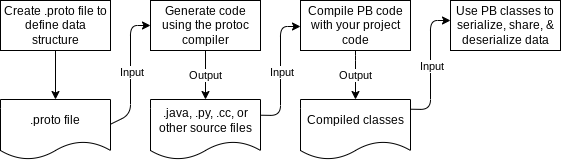
\includegraphics[width=0.8\textwidth]{images/protocol-buffers-concepts}
    \caption{Protocol Buffers Workflow~\cite{protobuf-overview}}
    \label{fig:protobuf-mechanism}
\end{figure}

There are two language versions of Protocol Buffers, version 2 and version 3.
The versions share the same basic concepts using the same syntax, but version 3 improves version 2 in several ways~\cite{protobuf-proto3}.
As this work focuses on the latest technologies, I will focus on version 3 of Protocol Buffers.
If no specific version is mentioned, it is assumed that version 3 is used.

\subsection{Structures}
The primary keywords in Protocol Buffers are \textit{message}, \textit{enum}, \textit{service}, \textit{method}, and \textit{package}.
The \textit{message} is used to define a data structure.
The \textit{enum} defines a set of named constants.
The \textit{service} is a set of \textit{methods} that can be called remotely.
And, the \textit{package} type is used to define a namespace for the defined \textit{messages}, \textit{enums}, and \textit{services}.
\cite{protobuf-proto3}

\subsubsection{Message}
Messages are used to define data structures.
They are defined using the \textit{message} keyword followed by the name of the message and a block of fields.
Each field has a name, a type, and a unique number across all fields in the \textit{message}.
The type of a field can be a scalar type or another \textit{message} type.
The possible scalar types are described in table~\ref{tab:protobuf-scalar-types} with their C++ counterparts.
The unique number is used to identify the field in the binary encoding.
Reusing the same number for different fields is therefore highly discouraged.
To avoid this, there is a \textit{reserved} keyword, which I will describe later.
\cite{protobuf-proto3}

\begin{table}[hbt!]
    \centering
    \captionsetup{justification=centering}
    \begin{tabular}{|l|l|}
        \hline
        .proto   & C++    \\ \hline
        double   & double \\ \hline
        float    & float  \\ \hline
        int32    & int32  \\ \hline
        int64    & int64  \\ \hline
        uint32   & uint32 \\ \hline
        uint64   & uint64 \\ \hline
        sint32   & int32  \\ \hline
        sint64   & int64  \\ \hline
        fixed32  & uint32 \\ \hline
        fixed64  & uint64 \\ \hline
        sfixed32 & int32  \\ \hline
        sfixed64 & int64  \\ \hline
        bool     & bool   \\ \hline
        string   & string \\ \hline
        bytes    & string \\ \hline
    \end{tabular}
    \caption{Scalar Types in Protocol Buffers~\cite{protobuf-proto3}}
    \label{tab:protobuf-scalar-types}
\end{table}

% Numbering
% Repeated
% Map
% Optional
% One Of
% Options
% reserved

Additional properties can be added to fields or types to alter their behavior.
The possibilities are \textit{reserved}, \textit{optional}, \textit{repeated}, \textit{map}, and \textit{oneof}.
\cite{protobuf-proto3}

The \textit{reserved} keyword is used to reserve a field number, preventing it from being used in the future.
This is useful when a field is removed from a message, and the field number should not be reused.
You can specify a single field number, a range of field numbers, or a list of field numbers and ranges.
\cite{protobuf-proto3}

In Protocol Buffers version 3, fields are inherently optional, with omitted fields assuming their default values.
This can create ambiguity when differentiating between a missing field and one explicitly set to its default.
The \textit{optional} keyword resolves this by providing a mechanism to explicitly mark fields as optional and track whether they have been set, even if the value is the default.
\cite{protobuf-proto3}

The \textit{repeated} keyword is used to define fields that can hold multiple values of the same type.
This is analogous to arrays or lists in common programming languages.
A repeated field allows you to represent collections of data within your message structure.
For example, a \textit{message} representing an order might have a \textit{repeated} field for line items, allowing multiple products within a single order.
Protocol Buffers offer efficient encoding mechanisms for repeated fields, making them suitable for representing ordered data lists.
\cite{protobuf-proto3}

The \textit{map} keyword is employed to define fields encompassing key-value pairs, akin to dictionaries or hashmaps in programming contexts.
A \textit{map} field allows the flexible association of related data without the constraints of a rigid structure.
For instance, a product attribute message could leverage a \textit{map} field where keys denote attribute names (``color'', ``size'') and their corresponding values provide the descriptions (``red'', ``large'').
\cite{protobuf-proto3}

Finally, the \textit{oneof} keyword provides a mechanism to define a message field where only one of several sub-fields can be set at a time.
This is valuable when the \textit{message} needs to represent mutually exclusive data variations.
For example, a payment\_method field within a \textit{message} could use a \textit{oneof} to support different payment types like credit\_card, debit\_card, or PayPal.
Setting one of these sub-fields automatically clears any previously set values within the \textit{oneof}.
This helps conserve memory and enforces a clear structure for alternative data representations.
\cite{protobuf-proto3}

\subsubsection{Enum}
Another type of structure is \textit{enum}.
It is used to define a set of named constants.
The constants are defined using the \textit{enum} keyword followed by the name of the \textit{enum} and a block of constants with their numeric values.
The special numeric value 0 is used as the default value.
Therefore, the first constant must have the value 0.
\cite{protobuf-proto3}

The \textit{enum} has a special option called \textit{allow\_alias}, which allows having the same numeric values for multiple names.
This is useful when the same value is used in different contexts.
\cite{protobuf-proto3}

\subsubsection{Service and Method}
The \textit{service} defines a set of \textit{methods} that can be called remotely.
It is defined using the \textit{service} keyword followed by the name of the \textit{service} and a block of \textit{methods}.
Each \textit{method} has a name, request, and response \textit{message} type.
The \textit{method} can also have a \textit{stream} keyword to define streaming of request, response, or both.
\cite{protobuf-proto3}

Streaming is a feature that allows the client and server to send a sequence of \textit{messages} back and forth until the stream is closed.
This is useful when the client or server needs to send a large number of \textit{messages} or just does not know the exact number of them in advance.
\cite{protobuf-proto3}

There are four types of gRPC calls.
When no streaming is involved, it is called \textit{unary} call.
When the request is streamed, it is called \textit{client-streaming} call.
When the response is streamed, it is called \textit{server-streaming} call.
And when both request and response are streamed, it is called \textit{bidirectional-streaming} call.
\cite{grpc-core-concept}

\subsubsection{Packages}
The \textit{package} is used to define a namespace for the defined \textit{messages}, \textit{enums}, and \textit{services} in the .proto file.
It is present at the beginning of the file using the \textit{package} keyword followed by the name of the \textit{package}.
The \textit{package} may not be considered for the code generation.
This is especially true for Java.
Because of that, a \textit{java\_package} option can be used to define the package for the generated code.
This option is defined at the file level.
\cite{protobuf-proto3}

The other option to differentiate \textit{messages} names is using nested types.
The \textit{message} can be defined inside another \textit{message}.
This is useful when the \textit{message} is used only in the context of the parent \textit{message} or is meaningful only in the parent \textit{message} context.
\cite{protobuf-proto3}

Both \textit{package} and nested types are used to avoid name conflicts and can be used using the dot notation between names.

\subsection{Comments}
The .proto files can contain comments.
The comments can be single-line or multi-line.
The single-line comments are started with the \textit{//} characters.
The multi-line comments start with the \textit{/*} characters and end with the \textit{*/} characters.
The comments can be used to describe the purpose of the \textit{message}, \textit{enum}, \textit{service}, \textit{method} or \textit{field}.
The comments can also describe the purpose of the \textit{package} or the whole file.
\cite{protobuf-proto3}

\subsection{Code Generation}
The .proto files generate the code for the specific programming language.
Code generation can be done using various tools, the recommended one being the Protocol Compiler (protoc).
It is used to generate the C++, C\#, Dart, Go, Java, Python, Ruby, and JavaScript code.
An example usage is described in the code snippet~\ref{lst:protobuf-protoc}.
Required classes and types are then generated, and the gRPC APIs can be called without extra coding work.
\cite{protobuf-proto3}

\begin{lstlisting}[language=bash, caption={Protocol Buffers Code Generation~\cite{protobuf-proto3}}, label={lst:protobuf-protoc}]
protoc --proto_path=IMPORT_PATH --java_out=DST_DIR path/to/file.proto
\end{lstlisting}

\subsection{Metadata}
Metadata are key-value pairs sent with the initial or final request or response.
They are used to provide additional information, such as authentication or tracing information.
Two types of metadata are used: headers and trailers.

Headers are sent before the initial client request and before the initial response from the server.
This applies only to the first message of the client and server.
The figure~\ref{fig:grpc-metadata} shows the gRPC headers in the request lifecycle.

\begin{figure}[hbt!]
    \centering
    \captionsetup{justification=centering}
    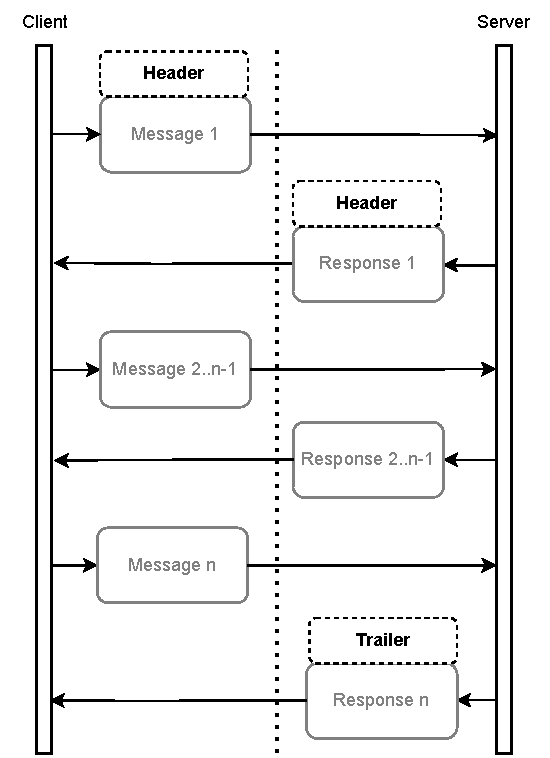
\includegraphics[width=0.4\textwidth]{images/grpc-metadata}
    \caption{gRPC Metadata}
    \label{fig:grpc-metadata}
\end{figure}

Trailers are sent after the server gives the final response.
They provide additional information about the response, such as the utilization or query cost.
The figure~\ref{fig:grpc-metadata} shows the gRPC trailers in the response lifecycle.

\cite{grpc-metadata}

\subsection{gRPC-web}
The gRPC is built on HTTP/2, using features like HTTP/2 framing~\cite{grpc-protocol-http2}.
As the HTTP/2 framing is not, and probably never be, directly exposed by any browser, the gRPC-Web protocol exists~\cite{grpc-protocol-web}.

The design goals of the gRPC-Web are:
\begin{itemize}
    \item to adopt the same framing as gRPC whenever possible,
    \item decouple from HTTP/2 framing,
    \item support text stream for cross-browser support~\cite{grpc-protocol-web}.
\end{itemize}

The gRPC-Web clients require a proxy, which is added between the client and the server.
The communication works as follows.
The browser sends a request to the proxy using the gRPC-Web protocol.
The proxy translates the gRPC-Web protocol to the gRPC protocol and sends the request to the server.
The server processes the request and sends the response back to the proxy.
The proxy translates the gRPC protocol to the gRPC-Web protocol and sends the response back to the browser.
The browser processes the response, and the communication is complete.
\cite{grpc-protocol-web}

The default proxy implementation is the Envoy\footnote{\url{https://www.envoyproxy.io/}} proxy.
It supports the gRPC-Web protocol out of the box.
Other options are, but not only, gRPC-web Go proxy\footnote{\url{https://github.com/improbable-eng/grpc-web/tree/master/go/grpcwebproxy}}, APISIX\footnote{\url{https://apisix.apache.org/blog/2022/01/25/apisix-grpc-web-integration/}}, and Nginx\footnote{\url{https://www.nginx.com/}}.

Because of the proxy and browser implementation, there are a few differences and current limitations of the gRPC-Web~\cite{grpc-web}.
The most important one is streaming support.
Currently, the gRPC-Web does not support client-side streaming (effectively bi-directional streaming).
It supports only unary calls and server-side streaming.
Based on the streaming roadmap, the client-side streaming is planned for the future.
It is planned for 2023+, but it has not been implemented yet~\cite{grpc-web-streaming-roadmap}.

\subsection{gRPC Reflection}
The gRPC protocol uses binary encoding.
Therefore, it is impossible to query the server without knowing the protobuf definition of the service and both request and response messages before the request.
The gRPC reflection is a way to get this information using a standardized gRPC service that allows other clients to query the server for the protobuf-defined APIs.
It includes all necessary information about the services, methods, enums, and messages.
This information can encode requests, query the server, and decode responses.
It is used by debugging tools such as grpcurl\footnote{\url{https://github.com/fullstorydev/grpcurl}}.
The gRPC reflection service is not exposed by default, so it must be explicitly enabled in the server configuration.
The support for it varies across different gRPC implementations in different programming languages.
\cite{grpc-reflection}


\section{Existing Documentation Tools}
This section examines popular tools for documenting gRPC, GraphQL, and RESTful APIs.
I'll assess the capabilities and shortcomings of each solution, addressing gRPC first, then GraphQL, and lastly, RESTful APIs.
The section will culminate in a summary of findings, a discussion of issues, and a proposed solution for the static web generator.

\subsection{Protocol Buffers}
In the Protocol Buffers world, there are several tools for generating documentation or interactive calls from the .proto files.
The most popular ones I have found are described in the following subsections.
% TODO: Write something more here

\subsubsection{Wombat}
Wombat is a cross-platform gRPC desktop app client.
The UI is in the figure~\ref{fig:grpc-wombat}.
It is used to call gRPC services and inspect the responses.
\cite{grpc-wombat}

\begin{figure}[hbt!]
    \centering
    \captionsetup{justification=centering}
    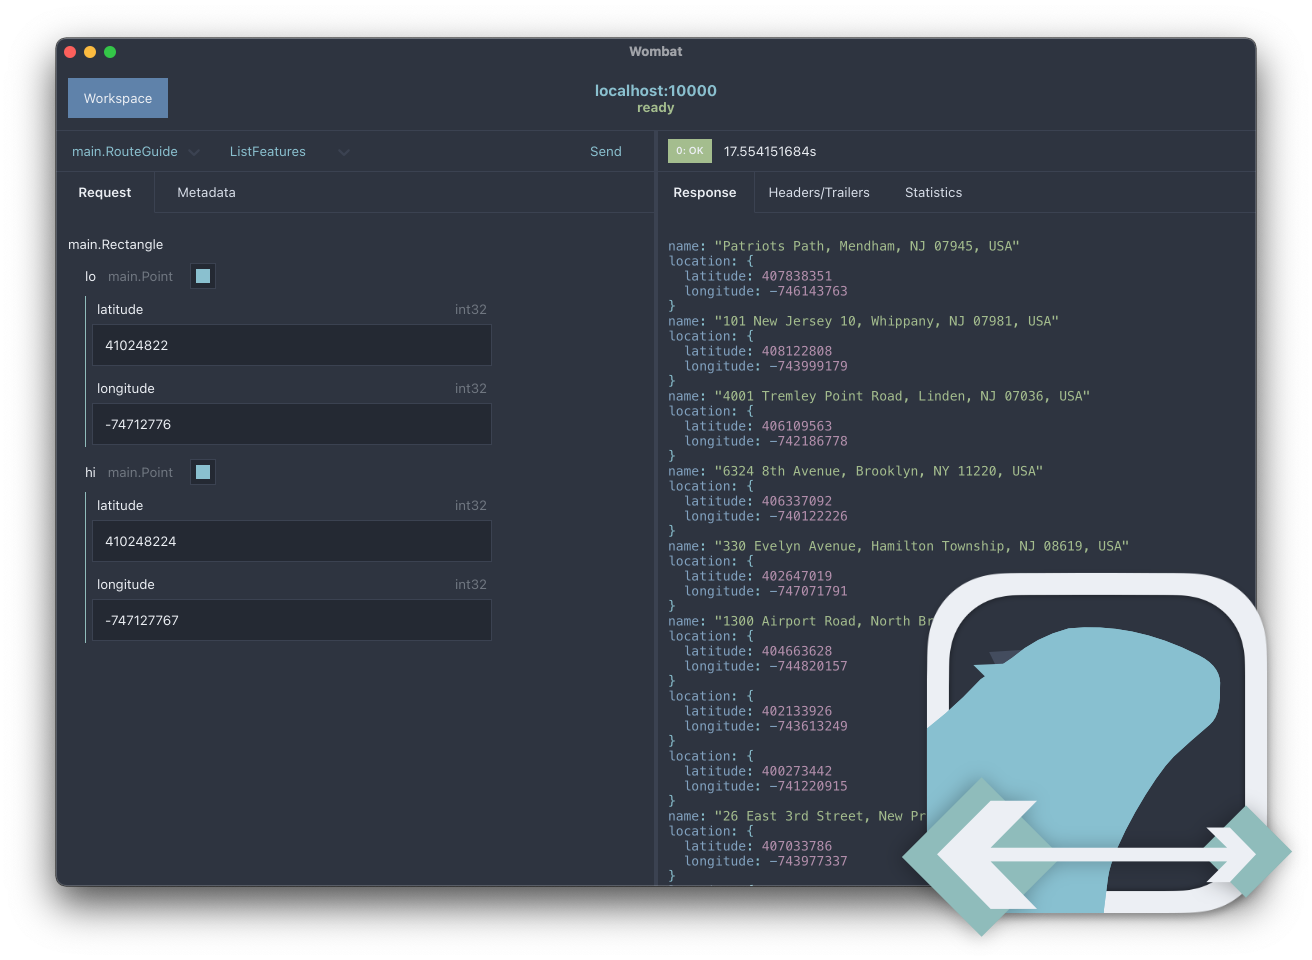
\includegraphics[width=0.8\textwidth]{images/grpc/wombat}
    \caption{Wombat GUI~\cite{grpc-wombat}}
    \label{fig:grpc-wombat}
\end{figure}

The main features are:
\begin{itemize}
    \item automatic parsing of proto definitions to render services and input messages,
    \item configuration of TLS,
    \item input form generation for all scalar types, nested messages, enums, repeated, oneof, and map,
    \item request metadata,
    \item execution of unary, server streaming, client streaming, bidirectional requests,
    \item pending request cancellation,
    \item sending EOF for client streaming,
    \item view response messages,
    \item view gRPC header and trailer,
    \item view RPC statistics,
    \item determine gRPC schema via reflection,
    \item support for Google Well Known Types,
    \item multiple workspace support~\cite{grpc-wombat}.
\end{itemize}

The main disadvantages (compared to my task) are:
\begin{itemize}
    \item desktop application (not a website),
    \item no support for documentation comments,
    \item last update 3 years ago~\cite{grpc-wombat}.
\end{itemize}

% Bugs: it doesn't remember the responses when you switch methods, UI is unfamiliar, a lot of errors even if you work with the software in a valid way

\subsubsection{BloomRPC}
BloomRPC is a cross-platform gRPC desktop app client.
The UI is in the figure~\ref{fig:grpc-bloomrpc}.
It is used to call gRPC services and inspect the responses.
\cite{grpc-bloomrpc}

\begin{figure}[hbt!]
    \centering
    \captionsetup{justification=centering}
    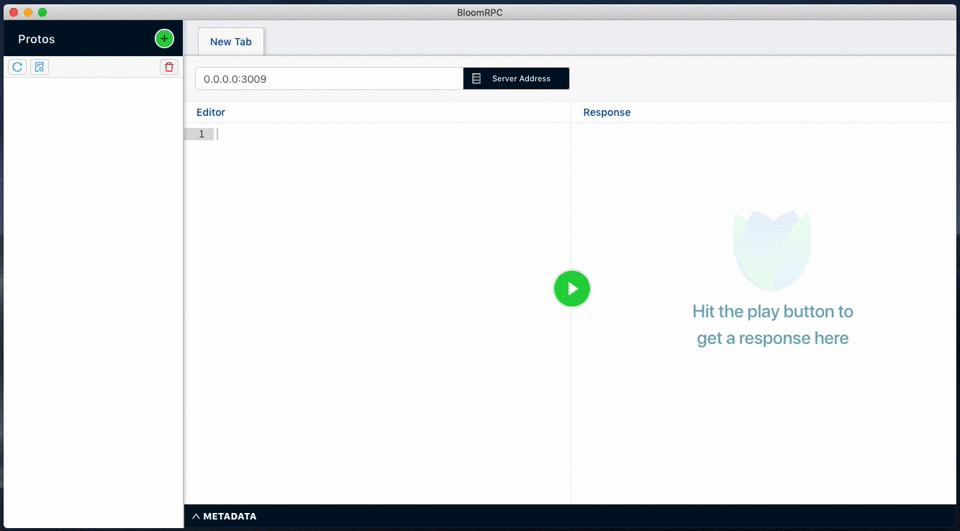
\includegraphics[width=0.8\textwidth]{images/grpc/bloomrpc}
    \caption{BloomRPC GUI~\cite{grpc-bloomrpc}}
    \label{fig:grpc-bloomrpc}
\end{figure}

The main features are:
\begin{itemize}
    \item automatic parsing of proto definitions to list services and example messages,
    \item configuration of TLS,
    \item request metadata,
    \item execution of unary, server streaming, client streaming, bidirectional requests,
    \item selection between gRPC and gRPC-Web,
    \item pending request cancellation,
    \item sending EOF for client streaming,
    \item view response messages~\cite{grpc-bloomrpc}.
\end{itemize}

The main disadvantages (compared to my task) are:
\begin{itemize}
    \item desktop application (not a website),
    \item no support for documentation comments,
    \item missing determine gRPC schema via reflection,
    \item missing gRPC headers and trailers preview,
    \item archived in 2023, usage is no longer recommended~\cite{grpc-bloomrpc}.
\end{itemize}

\subsubsection{gRPC Docs and GenDocu}
The gRPC Docs is a website API documentation generator by GenDocu.
It provides RPC calls documentation for gRPC services.
There is no option to call the services.
This documentation is generated from the .proto files using protoc-gen-doc\footnote{\url{https://github.com/pseudomuto/protoc-gen-doc}} utility with its custom format output as JSON\@.
The example web UI is in the figure~\ref{fig:grpc-gendocu}.
\cite{grpc-gendocu}

GenDocu is a hosted gRPC Docs version.
This version can call the gRPC services.
But, at the time of writing, the GenDocu website is not working anymore, and the project looks abandoned (with the last commit being more than a year ago).
\cite{grpc-gendocu}

\begin{figure}[hbt!]
    \centering
    \captionsetup{justification=centering}
    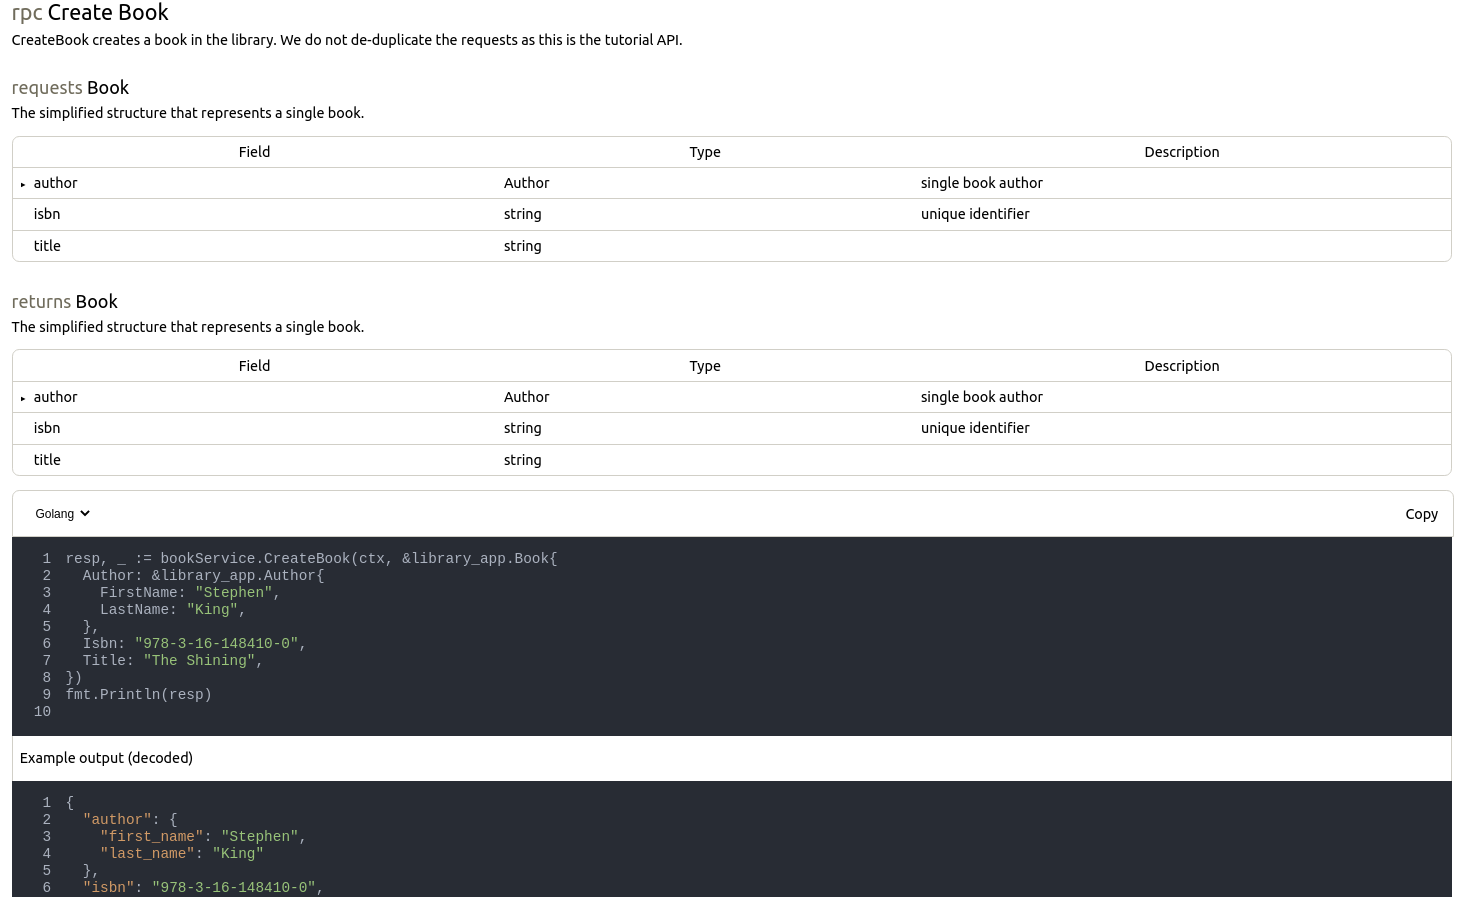
\includegraphics[width=0.8\textwidth]{images/grpc/gendocu}
    \caption{GenDocu Web UI~\cite{grpc-gendocu}}
    \label{fig:grpc-gendocu}
\end{figure}

The main features are:
\begin{itemize}
    \item .proto files parsing and services, messages, enums generation,
    \item support for documentation comments,
    \item generation using common JSON format with the ability to change the source without redeploying the website~\cite{grpc-gendocu}.
\end{itemize}

The main disadvantages (compared to my task) are:
\begin{itemize}
    \item missing determine gRPC schema via reflection,
    \item execution of unary, server streaming, client streaming, bidirectional requests,
    \item inactive and looks abandoned with no external websites working~\cite{grpc-gendocu}.
\end{itemize}

\subsubsection{gRPC UI}
The gRPC UI is a website that supports calling gRPC services.
With this tool, you can browse the schema, which is presented as a list of available endpoints.
The schema can be constructed by querying a server that supports server reflection, reading proto source files, or loading a compiled `protoset' file (files containing an encoded file descriptor protos).
The protoset file can be created using the protoc tool, which is used by the gRPC tooling for the client's code generation.
The UI is in the figure~\ref{fig:grpc-grpcui}.
\cite{grpc-grpcui}

\begin{figure}[hbt!]
    \centering
    \captionsetup{justification=centering}
    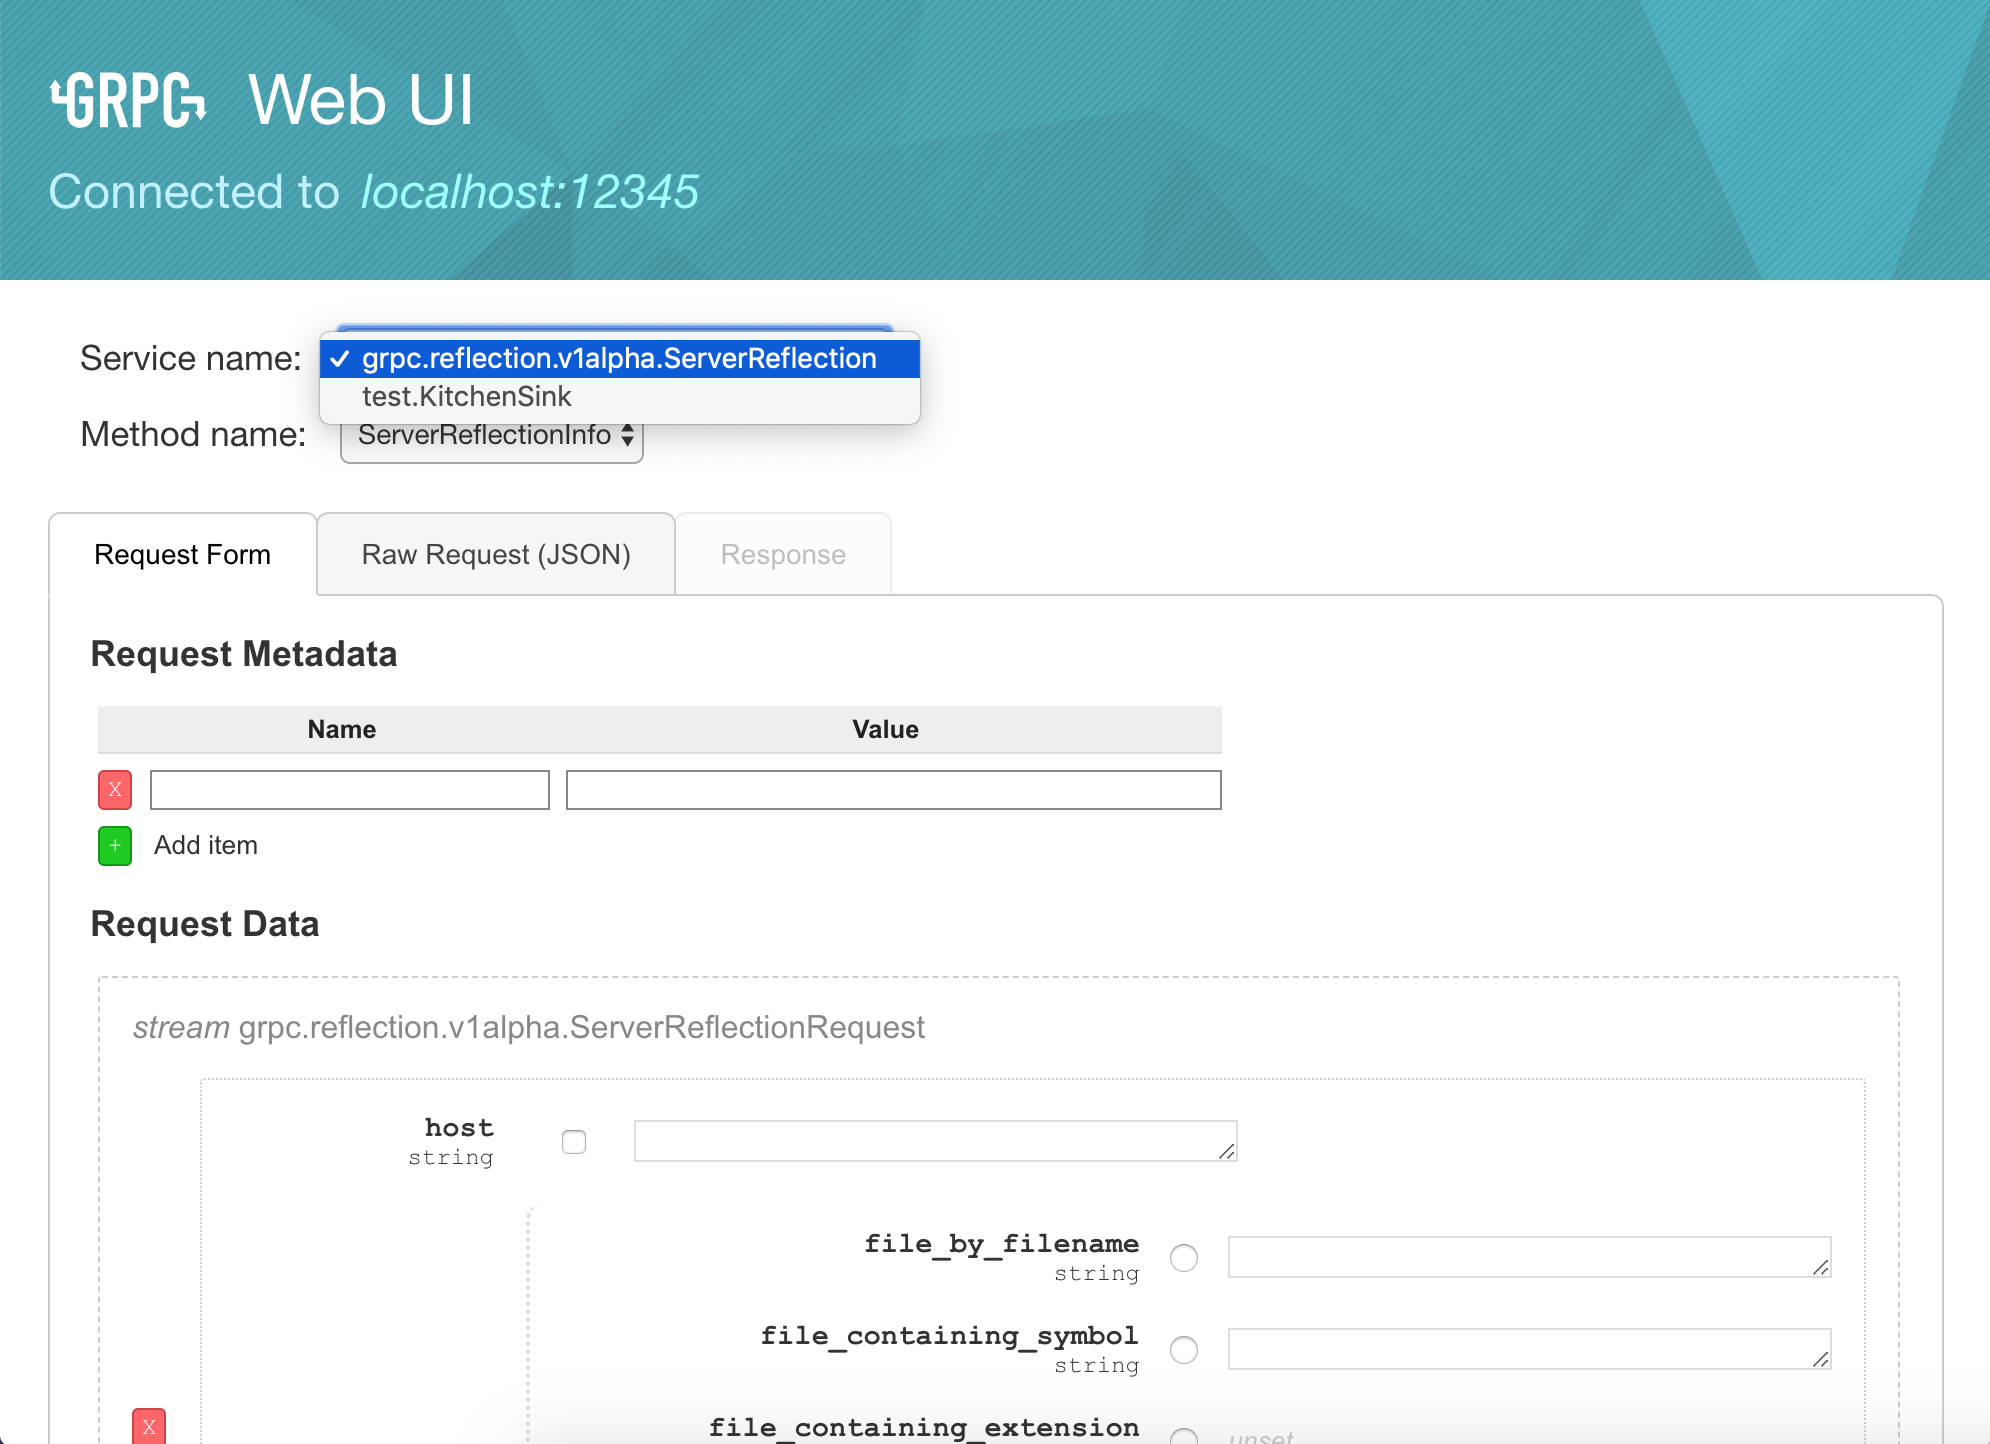
\includegraphics[width=0.8\textwidth]{images/grpc/grpcui}
    \caption{gRPC UI~\cite{grpc-grpcui}}
    \label{fig:grpc-grpcui}
\end{figure}

The main features are:
\begin{itemize}
    \item listing services and methods,
    \item ability to construct messages with forms or raw JSON,
    \item execution of unary, server streaming, client streaming, bidirectional requests,
    \item request metadata, headers and trailers,
    \item configuration of TLS,
    \item rich support for well-known types,
    \item view response messages,
    \item actively maintained~\cite{grpc-grpcui}.
\end{itemize}

The main disadvantages (compared to my task) are:
\begin{itemize}
    \item requires a server to run (not a static website),
    \item no support for documentation comments,
    \item requires you to construct the entire stream of request messages all at once, and then it shows the entire resulting stream of response messages all at once (so you can't interact with any streams interactively)~\cite{grpc-grpcui}.
\end{itemize}

\subsubsection{letmegrpc}
The gRPC UI is a website that supports calling gRPC services.
It allows service methods to call using forms, where each method has its separate URL (\url{http://localhost:8080/ServiceName/MethodName}).
It is constructed from a .proto file.
The UI is in the figure~\ref{fig:grpc-letmegrpc}.
\cite{grpc-letmegrpc}

\begin{figure}[hbt!]
    \centering
    \captionsetup{justification=centering}
    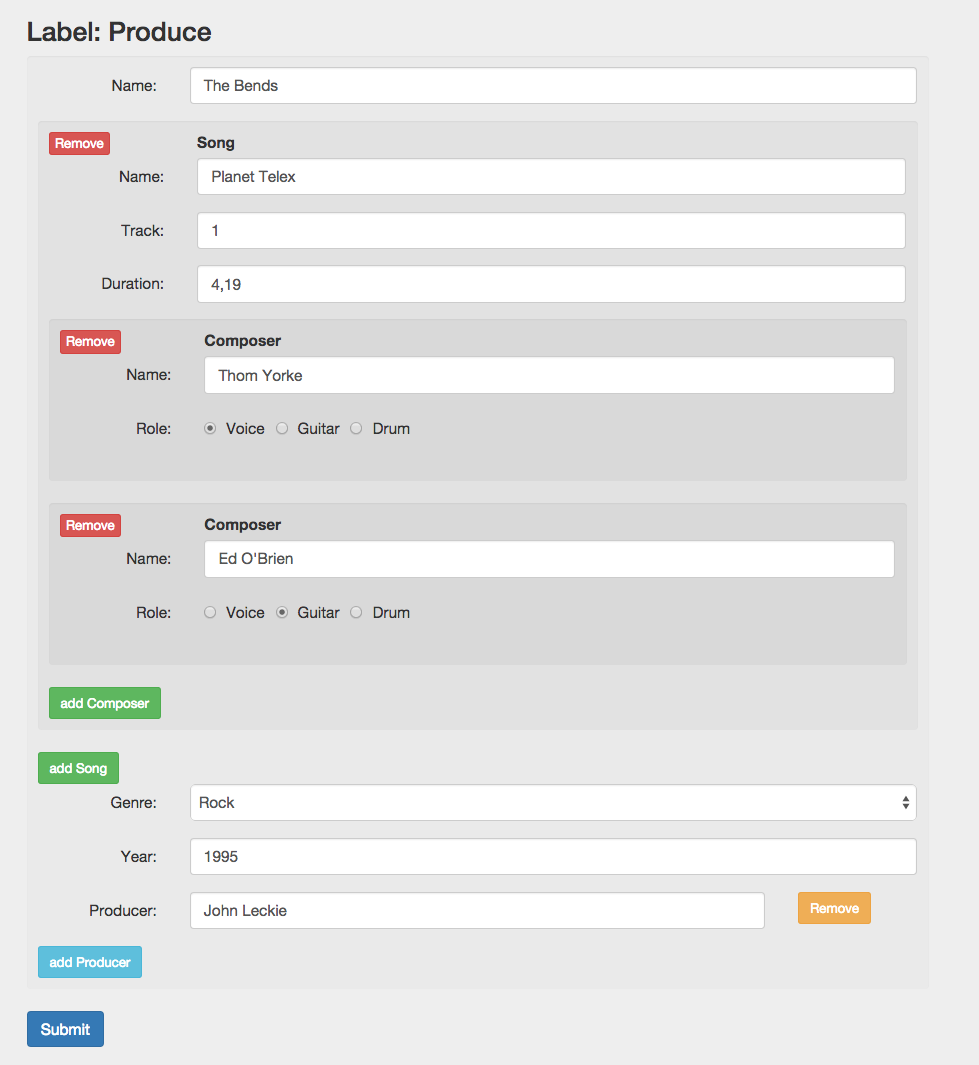
\includegraphics[width=0.8\textwidth]{images/grpc/letmegrpc}
    \caption{letmegrpc UI~\cite{grpc-letmegrpc}}
    \label{fig:grpc-letmegrpc}
\end{figure}

The main features are:
\begin{itemize}
    \item comments to fields are in tooltips,
    \item ability to construct messages with forms,
    \item execution of unary, server streaming, client streaming, bidirectional requests,
    \item view response messages~\cite{grpc-letmegrpc}.
\end{itemize}

The main disadvantages (compared to my task) are:
\begin{itemize}
    \item requires setup with manual go package downloads,
    \item no listing of services and methods,
    \item requires a server to run (not a static website),
    \item even though forms are powerful, they can be annoying to use, especially with complex requests,
    \item no support for request metadata, headers, and trailers,
    \item no direct support for gRPC reflection,
    % TODO: Correct citation?
    \item custom proto file parser, which does not have implemented all language features (\cite{grpc-letmegrpc-issue44}),
    \item inactive, the last update was five years ago~\cite{grpc-letmegrpc}.
\end{itemize}

\subsubsection{gRPC-swagger}
The gRPC Swagger is a website.
It is based on gRPC reflection and can list and call gRPC services.
It uses Swagger UI design language (copy of the Swagger UI) but is not a part of the official Swagger.
The UI is in the figure~\ref{fig:grpc-swagger}.
The architecture is done using its server as a proxy.
The website's server forwards all requests to the gRPC server and back to the website.
\cite{grpc-letmegrpc}

\begin{figure}[hbt!]
    \centering
    \captionsetup{justification=centering}
    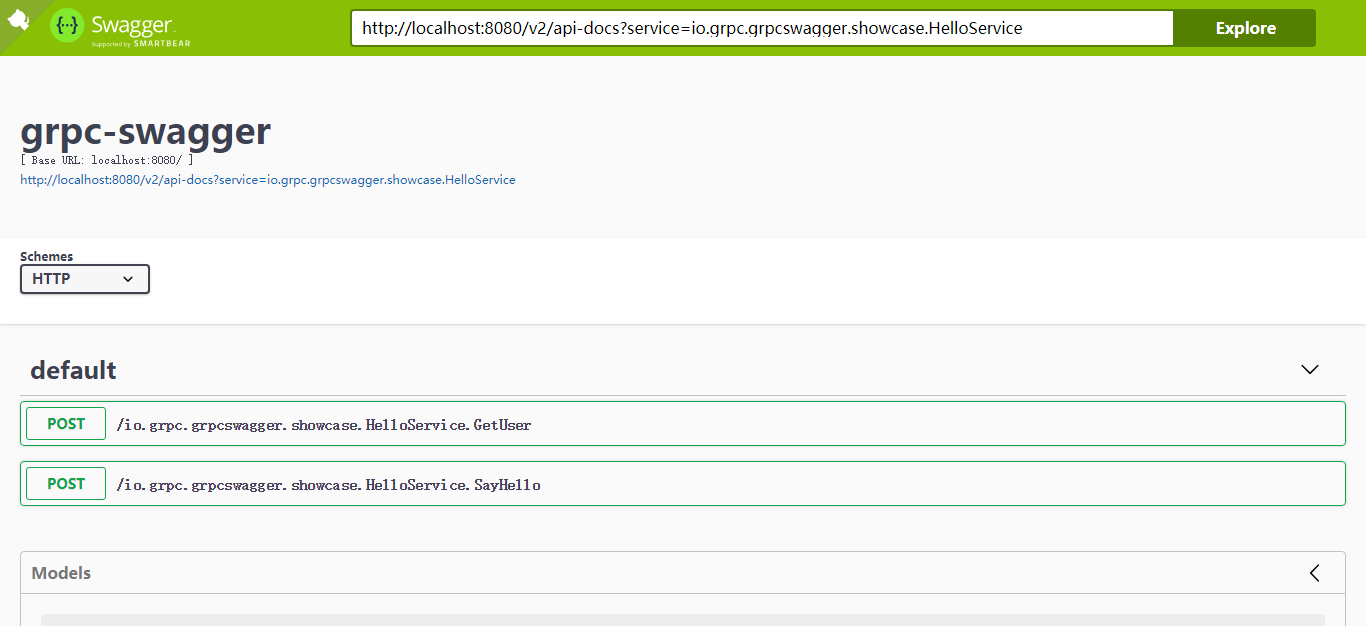
\includegraphics[width=0.8\textwidth]{images/grpc/swagger-1}
    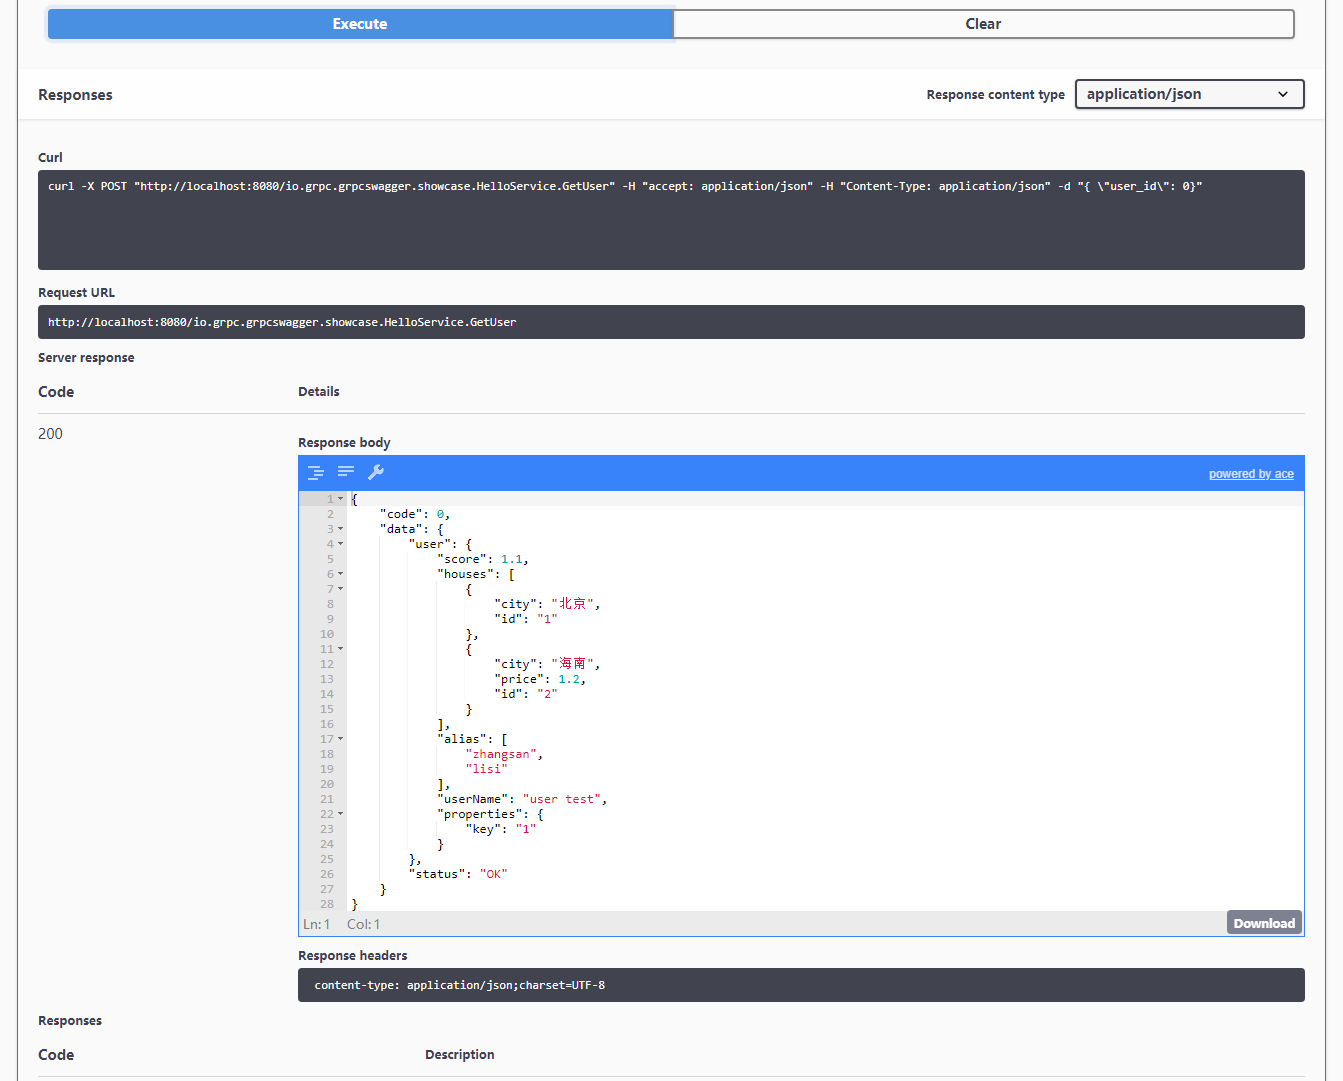
\includegraphics[width=0.8\textwidth]{images/grpc/swagger-2}
    \caption{gRPC Swagger UI~\cite{grpc-swagger}}
    \label{fig:grpc-swagger}
\end{figure}

The main features are:
\begin{itemize}
    \item listing of services and methods,
    \item familiar UI to the Swagger UI,
    \item support for request metadata, headers, and trailers,
    \item execution of unary, server streaming, client streaming, bidirectional requests,
    \item view response messages~\cite{grpc-swagger}.
\end{itemize}

The main disadvantages (compared to my task) are:
\begin{itemize}
    \item requires reflection enabled,
    \item no support for comments,
    \item requires a server to run (not a static website),
    \item it requires to construct the entire stream of request messages all at once, and then it shows the entire resulting stream of response messages all at once (so you can't interact with any streams interactively)
    \item request data are only in the form of JSON,
    \item inactive, last update two years ago, last release in 2020~\cite{grpc-swagger}.
\end{itemize}

\subsubsection{gRPC-Gateway}
The gRPC-Gateway is a protoc compiler plugin.
It generates a reverse proxy server, translating a RESTful JSON API into gRPC\@.
So, it is a reverse proxy server, not a documentation website, nor a client for calling gRPC\@.
It can also generate OpenAPI definitions using protoc-gen-openapiv2, which can be used with tools like Swagger UI\@.
\cite{grpc-letmegrpc}

It uses annotations in the service definitions or a configuration file.
An example of annotation is in the code snippet~\ref{lst:grpc-gateway-annotations},
and an example of the configuration file is in the code snippet~\ref{lst:grpc-gateway-configuration}.
\cite{grpc-letmegrpc}


\begin{lstlisting}[language=protobuf2, style=protobuf, caption={gRPC-Gateway Annotations~\cite{grpc-gateway}}, label={lst:grpc-gateway-annotations}]
import "google/api/annotations.proto";

rpc Echo(StringMessage) returns (StringMessage) {
  option (google.api.http) = {
    post: "/v1/example/echo"
    body: "*"
  };
}
\end{lstlisting}

\begin{lstlisting}[style=yaml, caption={gRPC-Gateway Configuration File~\cite{grpc-gateway}}, label={lst:grpc-gateway-configuration}]
type: google.api.Service
config_version: 3

http:
  rules:
    - selector: your.service.v1.YourService.Echo
      post: /v1/example/echo
      body: "*"
\end{lstlisting}

The main features are:
\begin{itemize}
    \item support for request metadata, headers,
    \item ability to create OpenAPI definitions,
    \item execution of unary, server streaming, client streaming, bidirectional requests, but in a batched manner,
    \item and much more regards the specifics of the reverse-proxy layer~\cite{grpc-gateway}.
\end{itemize}

The main disadvantages (compared to my task) are:
\begin{itemize}
    \item dependent on OpenAPI/HTTP API - is not just a gRPC client, but much more,
    \item OpenAPI definitions do not have to reflect the gRPC service definitions,
    \item no support for trailers,
    \item no support for true bi-directional streaming,
    \item requires the underline gRPC service definitions,
    \item no support for reflection,
    \item no support for documentation/comments,
    \item requires a server to run (not a static website)~\cite{grpc-gateway}.
\end{itemize}

\subsubsection{Postman}
Postman is the leading API platform~\cite{postman-popularity}.
It supports many different API types (e.g.,\ HTTP API, WebSockets, GraphQL) but also includes gRPC\@.
Upon loading .proto files or using gRPC reflection, it can understand the gRPC API and use the information for calls.
It can do more than call the gRPC services, but it is not a documentation website.
So, I will focus on its gRPC capabilities.
The UI is in the figure~\ref{fig:postman}.
\cite{postman}

\begin{figure}[hbt!]
    \centering
    \captionsetup{justification=centering}
    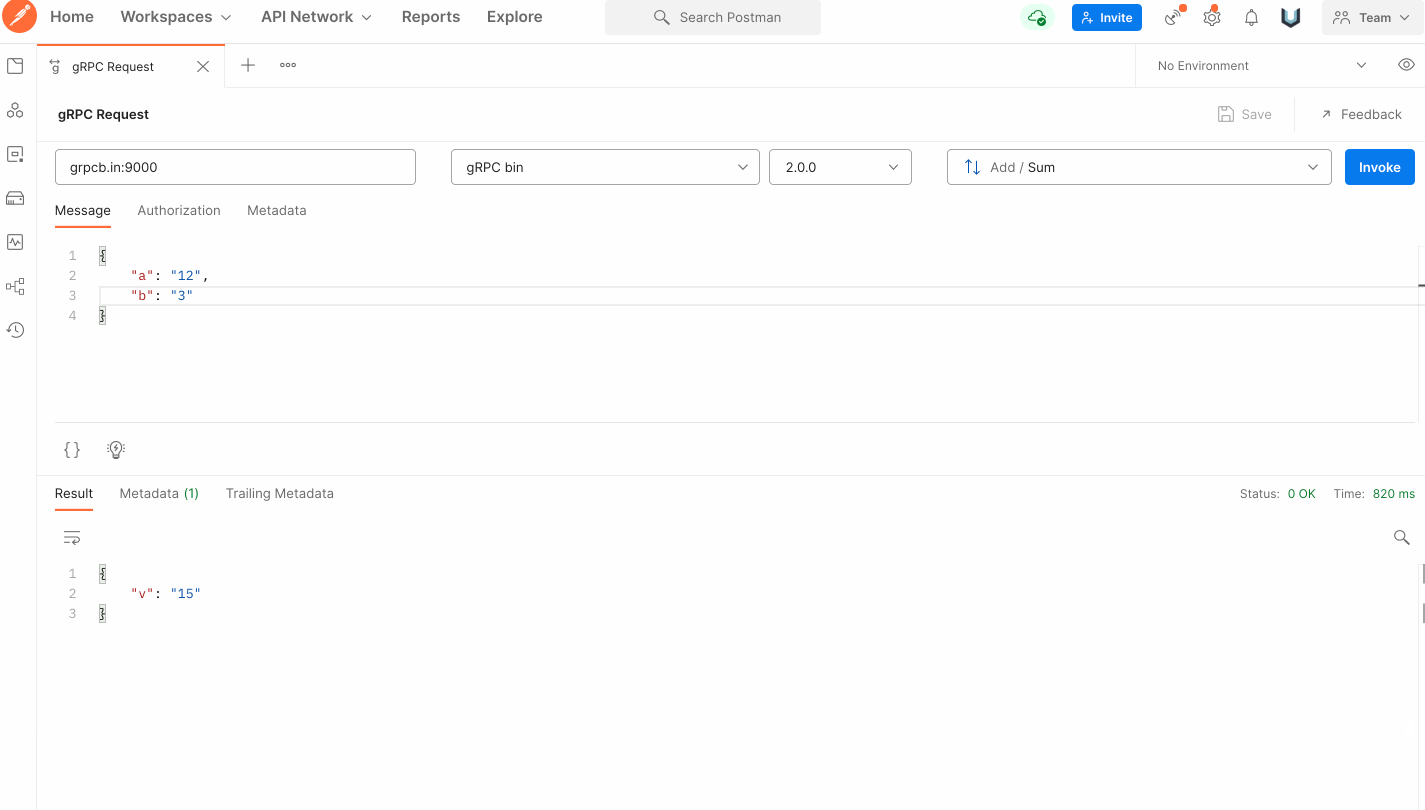
\includegraphics[width=0.8\textwidth]{images/postman}
    \caption{Postman UI~\cite{postman}}
    \label{fig:postman}
\end{figure}

The main features are:
\begin{itemize}
    \item listing of services and methods,
    \item execution of unary, server streaming, client streaming, bidirectional requests,
    \item broad range of features for API calls, including automated tests,
    \item support for request metadata, headers, and trailers,
    \item supports gRPC reflection,
    \item messages autocompletion,
    \item messages validation,
    \item view response messages with full support for streaming~\cite{postman}.
\end{itemize}

The main disadvantages (compared to my task) are:
\begin{itemize}
    \item it is a desktop application, not a static website,
    \item no support for comments,
    \item request data are only in the form of JSON~\cite{postman}.
\end{itemize}

\subsubsection{proto2asciidoc}
The proto2asciidoc is a plugin for the protoc tool that generates AsciiDoc documentation.
Many tools can then parse the AsciiDoc format.
One of these tools can be a static website.
The main disadvantage is that it is not a website or application but a documentation file.
Therefore, it does not allow calling the gRPC services at all.
Another disadvantage is the special comment block formatting requirement, which differs from usual comments in proto files.
And finally, it looks to be abandoned with the last commit more than two years ago.
\cite{grpc-proto2asciidoc}

\subsubsection{protoc-gen-doc}
A documentation generator for the protoc compiler tool.
It can generate HTML, JSON, DocBook, and Markdown documentation from comments in .proto files.
The main advantages are that it can take comments from the .proto files and generate a static documentation website or JSON, keeping the original structure of the input .proto files.
The website contains the documentation of the services, methods, and messages.
The JSON can then be used to create a custom website. For example, GenDocu mentioned earlier uses it.
The disadvantage is that it does not allow the gRPC services to be called.
\cite{grpc-protoc-gen-doc}

% Example website: https://rawgit.com/pseudomuto/protoc-gen-doc/master/examples/doc/example.html

\subsection{GraphQL}
In the GraphQL world, there are several tools for generating documentation or interactive calls.
The most popular ones based on the state of GraphQL in 2022 and others I have found for documentation are in the following subsections~\cite{graphql-popularity}.

\subsubsection{graphdoc}
GraphDoc is a static website generator for GraphQL schemas.
It supports live endpoint and .graphql definition files.
The generated website contains the documentation of the queries, mutations, and types.
They are shown in a file-like structure with interactive-type definition links.
The UI is in the figure~\ref{fig:graphql-graphdoc}.
\cite{graphql-graphdoc}

\begin{figure}[hbt!]
    \centering
    \captionsetup{justification=centering}
    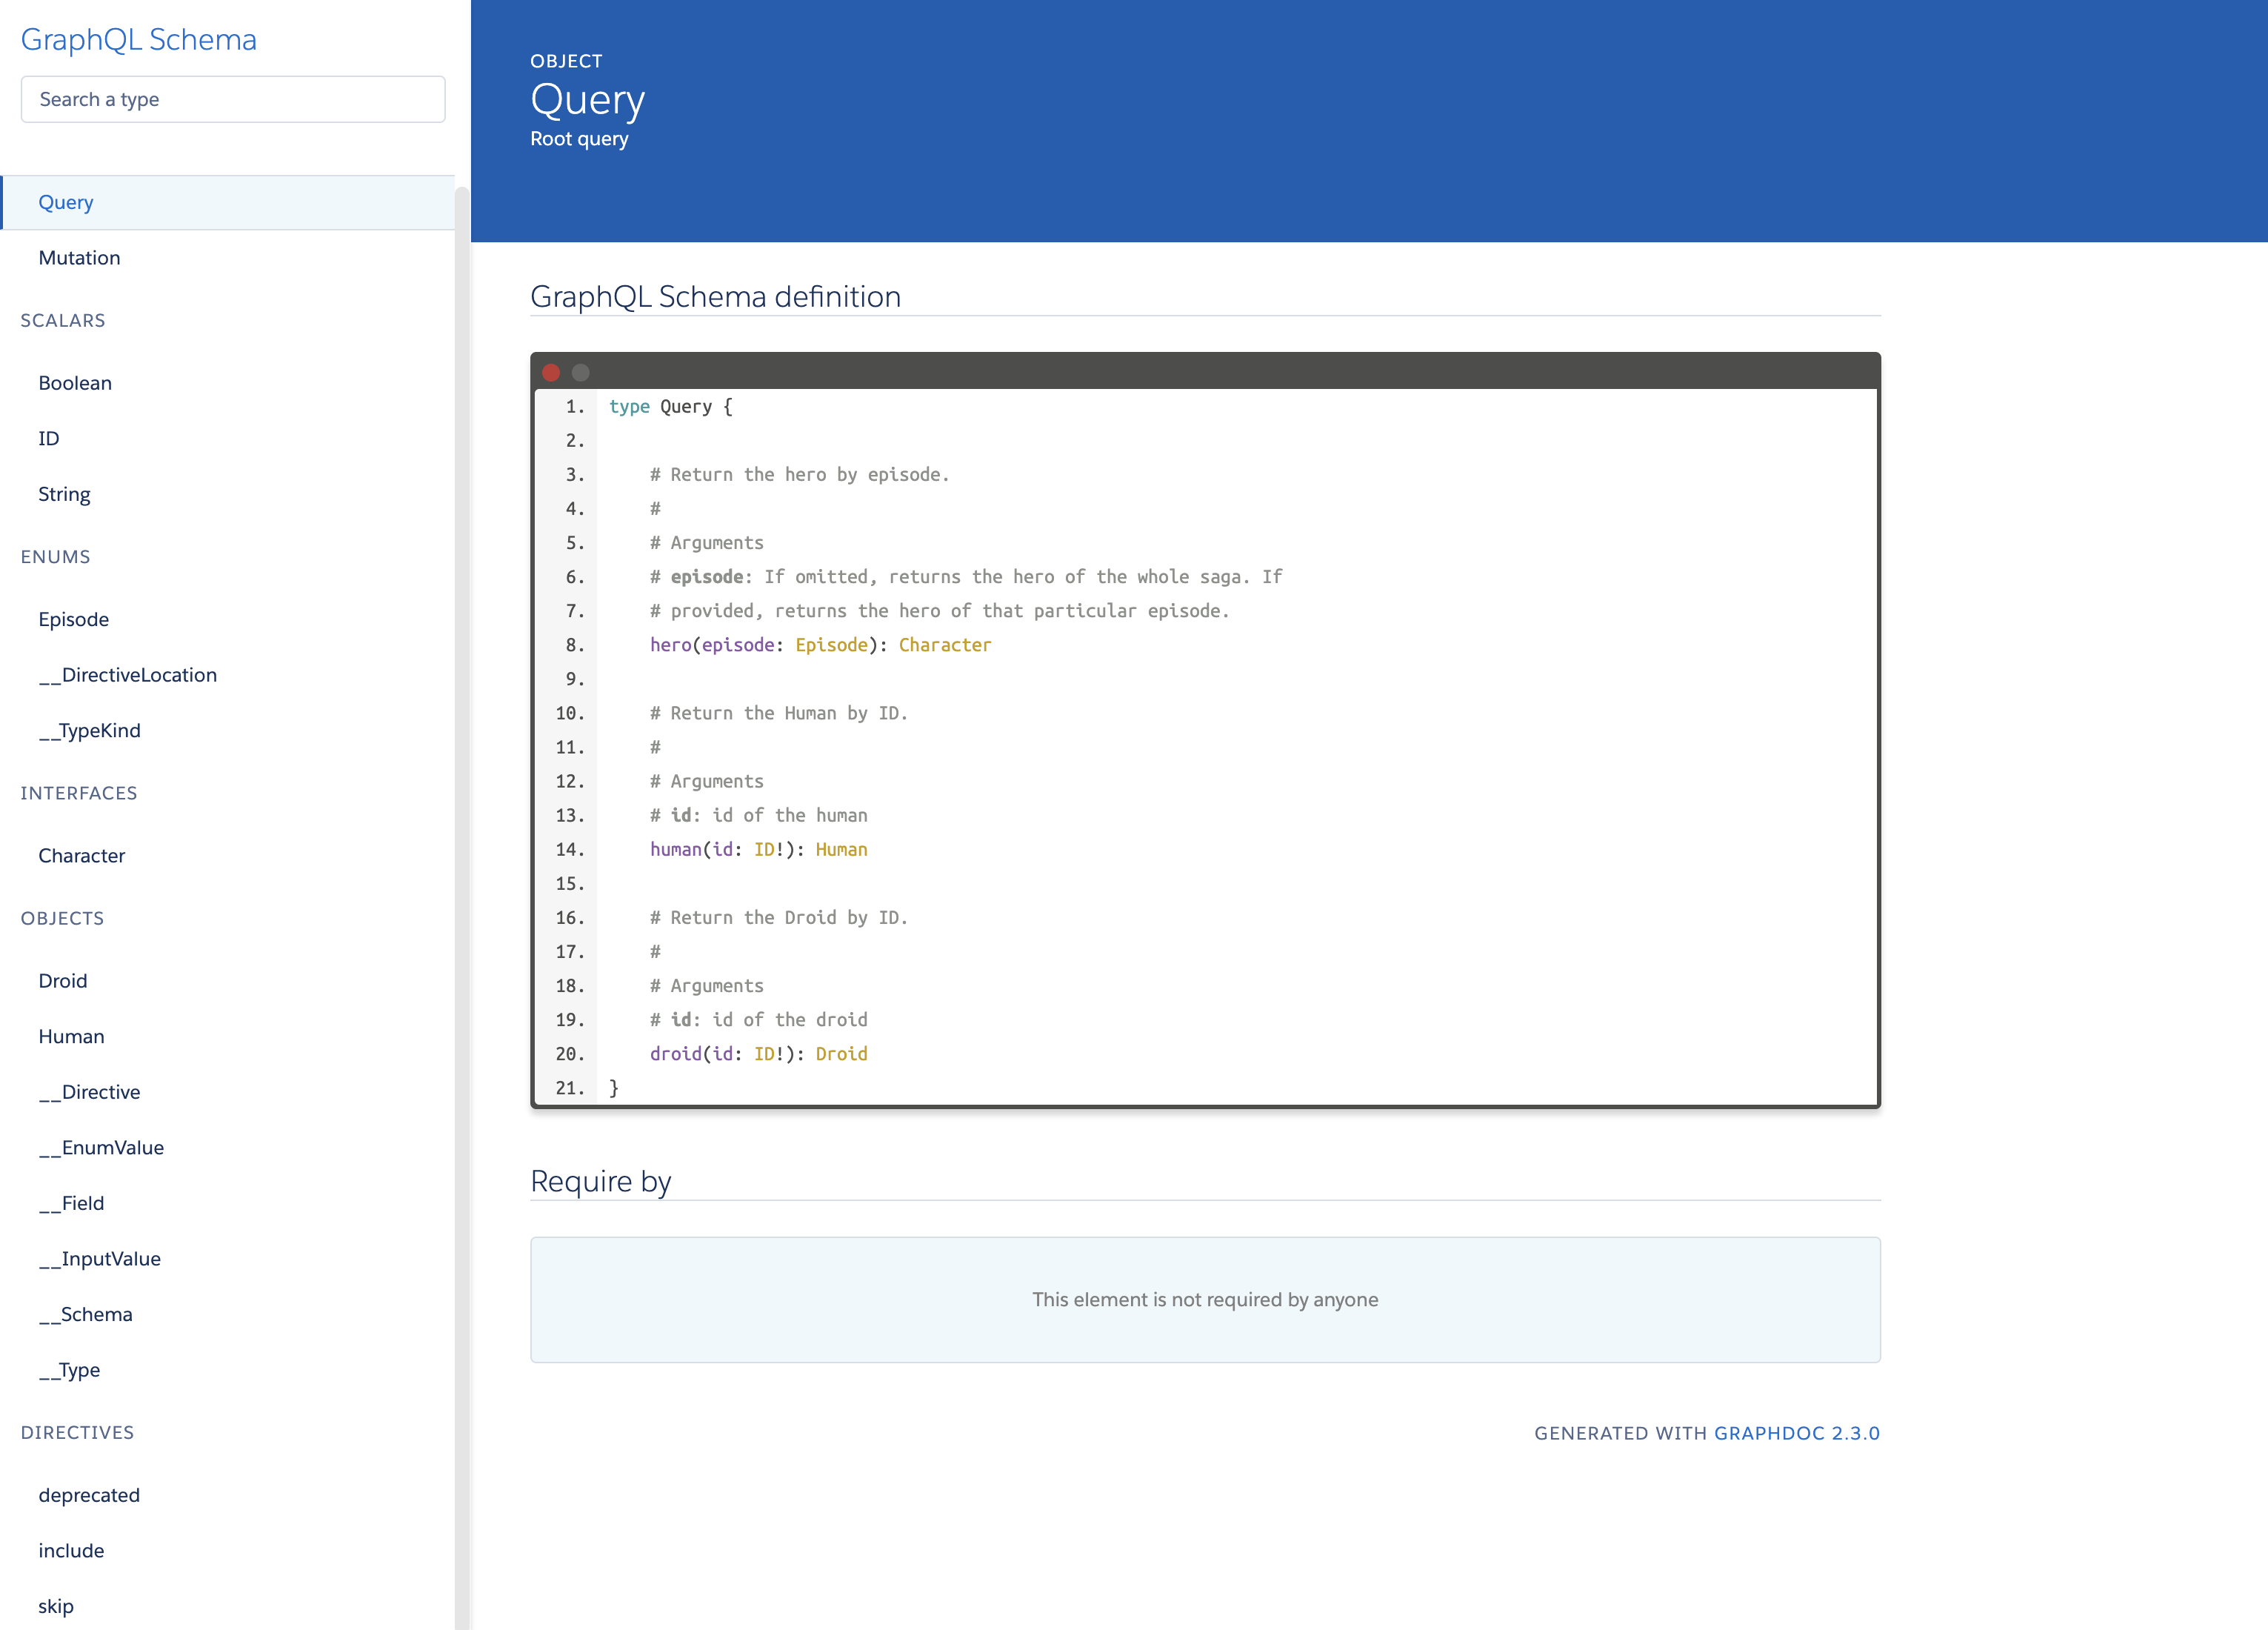
\includegraphics[width=0.8\textwidth]{images/graphql/graphdoc}
    \caption{GraphDoc UI~\cite{graphql-graphdoc}}
    \label{fig:graphql-graphdoc}
\end{figure}

The main features are:
\begin{itemize}
    \item static website,
    \item listing of queries, mutations, and types,
    \item generation from the live endpoint and .graphql definition files,
    \item documenting comments~\cite{graphql-graphdoc}.
\end{itemize}

The main disadvantages (compared to my task) are:
\begin{itemize}
    \item no requests execution,
    \item not actively maintained (last commit three years ago)~\cite{graphql-graphql-playground}.
\end{itemize}

\subsubsection{GraphQL Playground}
GraphQL Playground is an application for desktop and web.
It allows developers to build and test GraphQL queries and mutations, explore an API schema, and view real-time results.
GraphQL Playground offers features like automatic schema documentation, query history, and support for GraphQL subscriptions.
It uses a live endpoint and can be hosted as a static website.
The UI is in the figure~\ref{fig:graphql-graphql-playground}.
\cite{graphql-graphql-playground}

\begin{figure}[hbt!]
    \centering
    \captionsetup{justification=centering}
    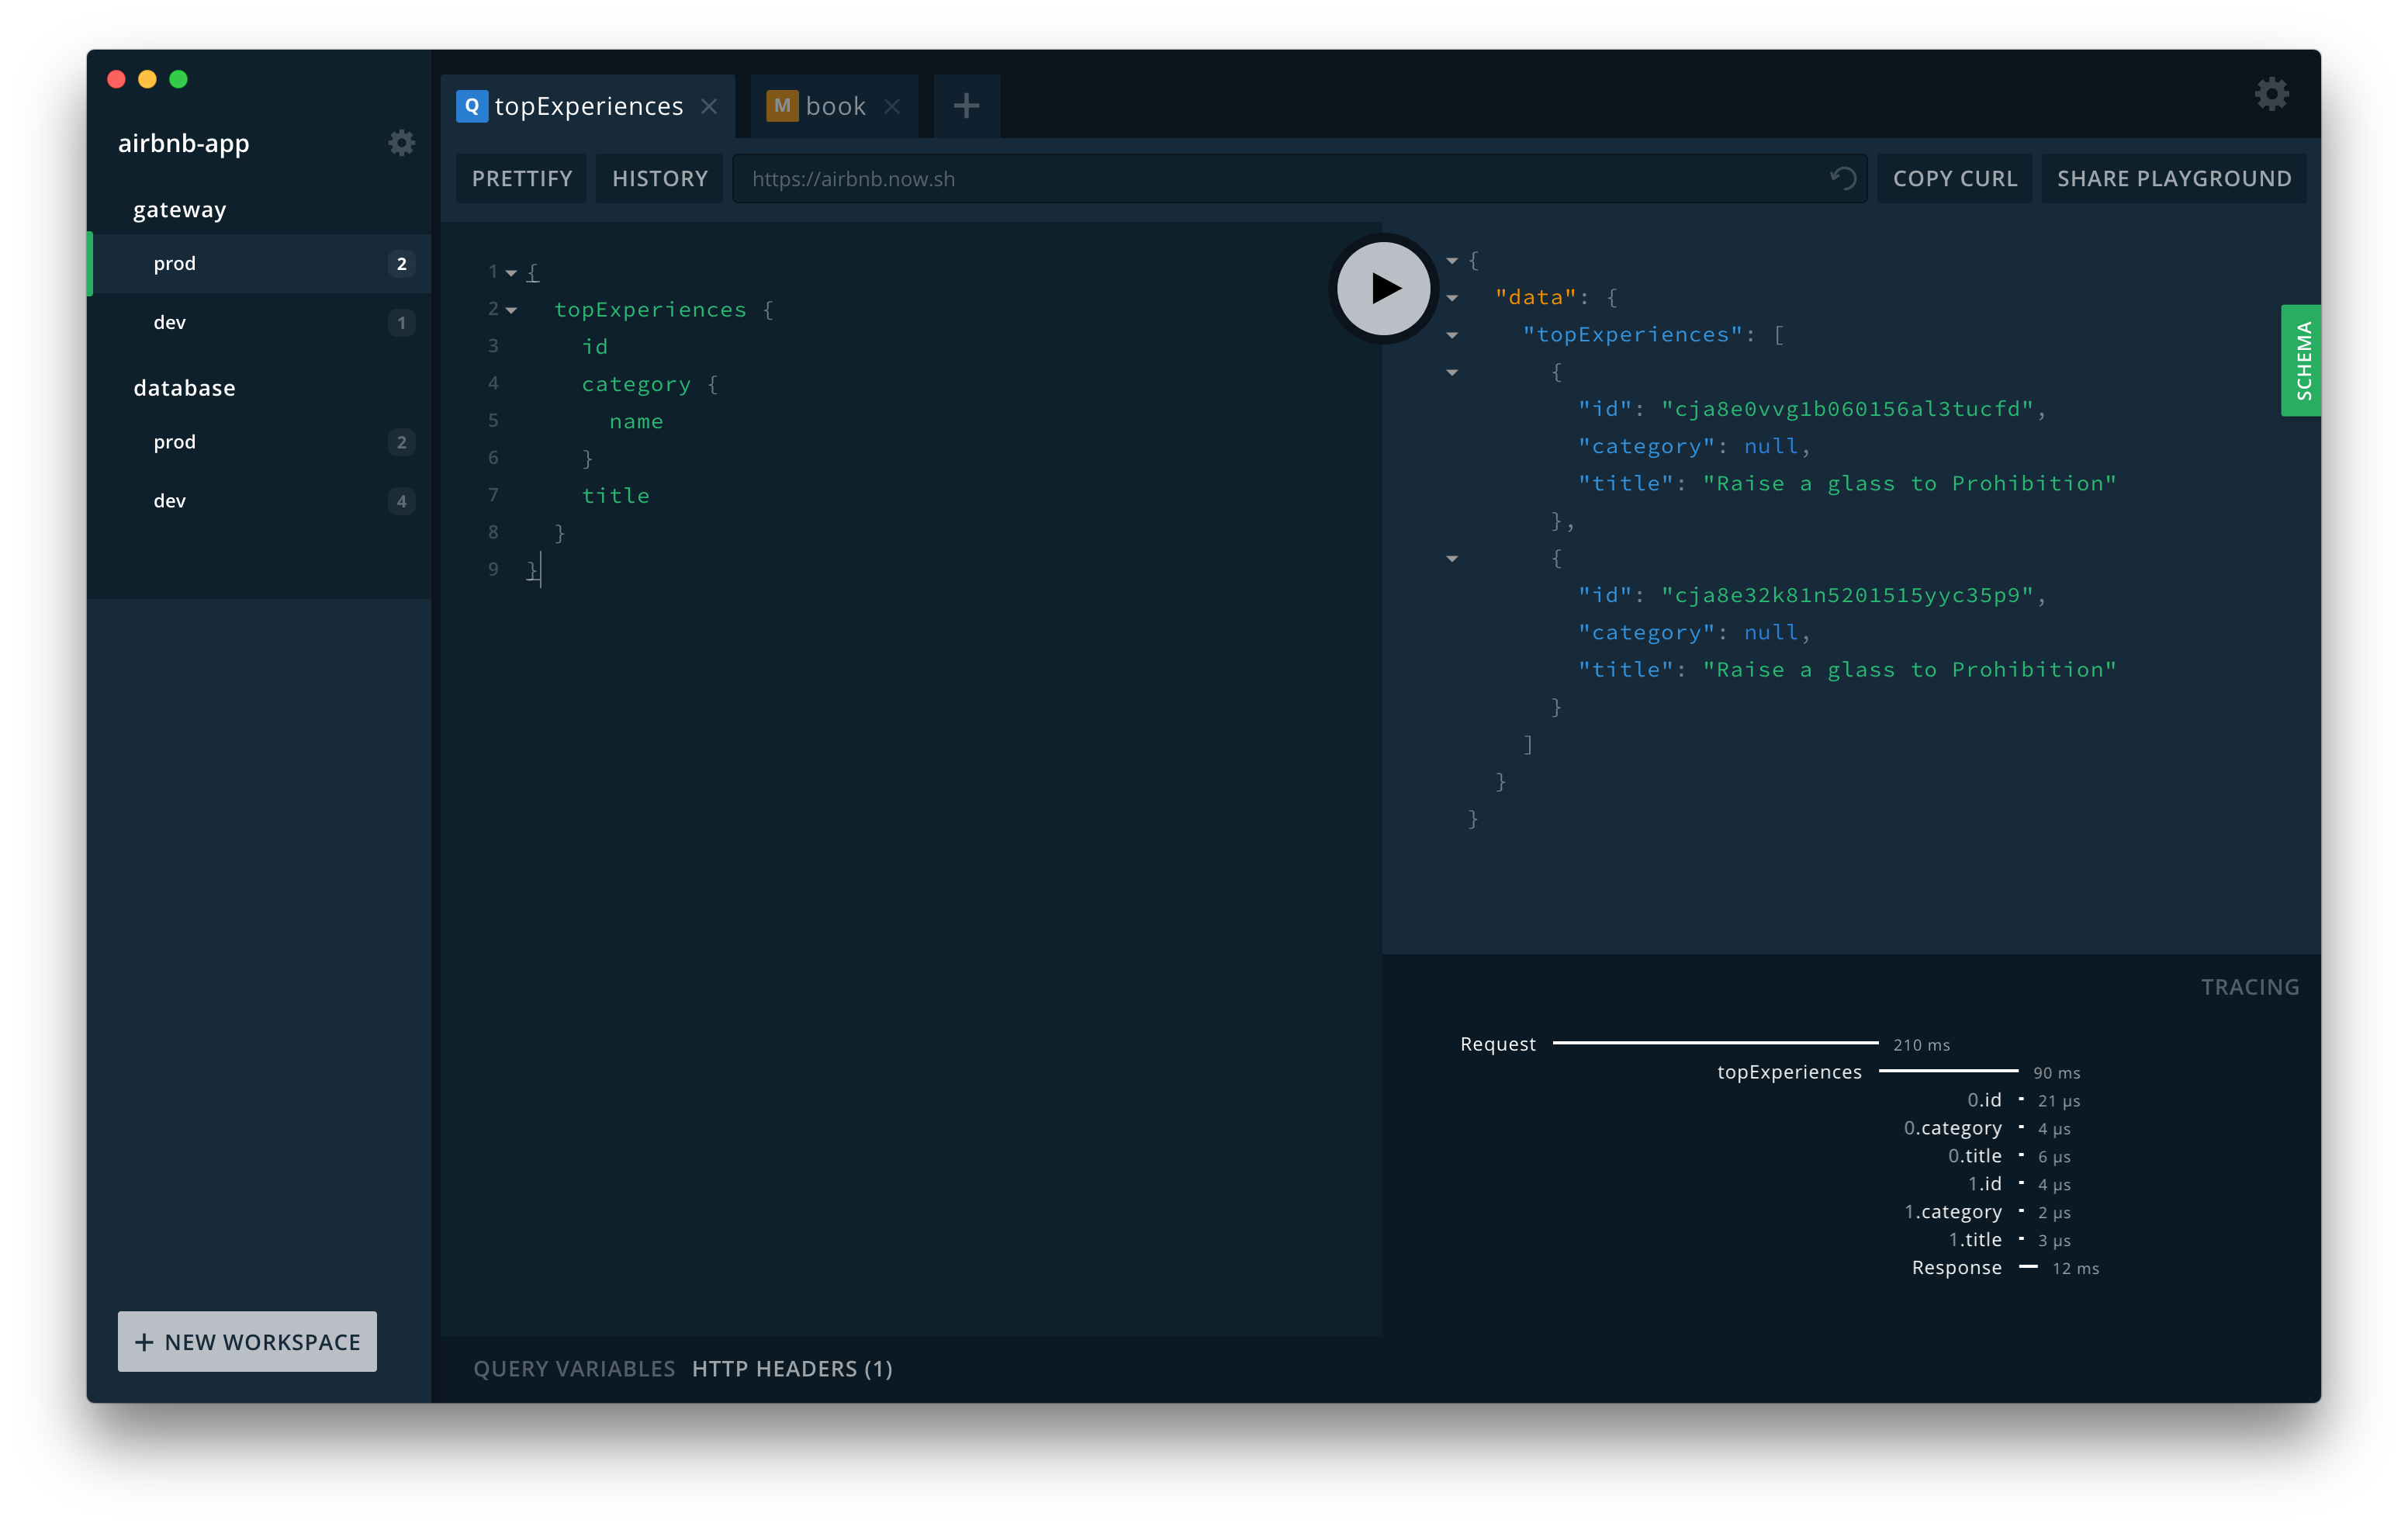
\includegraphics[width=0.8\textwidth]{images/graphql/graphql-playground}
    \caption{GraphQL Playground UI~\cite{graphql-graphql-playground}}
    \label{fig:graphql-graphql-playground}
\end{figure}

The main features are:
\begin{itemize}
    \item context-aware autocompletion,
    \item listing of queries, mutations, and types,
    \item real-time GraphQL subscriptions,
    \item multiple projects and endpoints support,
    \item can be static website~\cite{graphql-graphql-playground}.
\end{itemize}

The main disadvantages (compared to my task) are:
\begin{itemize}
    \item no documenting comments,
    \item not actively maintained (last commit two years ago, the last release in 2019)~\cite{graphql-graphql-playground}.
\end{itemize}

\subsubsection{GraphiQL}
GraphiQL is an interactive in-browser IDE\@.
It allows GraphQL API documentation exploring and the ability to execute queries and mutations.
It takes an endpoint and generates a static website.
The UI is in the figure~\ref{fig:graphql-graphiql}.
\cite{graphql-graphiql}

\begin{figure}[hbt!]
    \centering
    \captionsetup{justification=centering}
    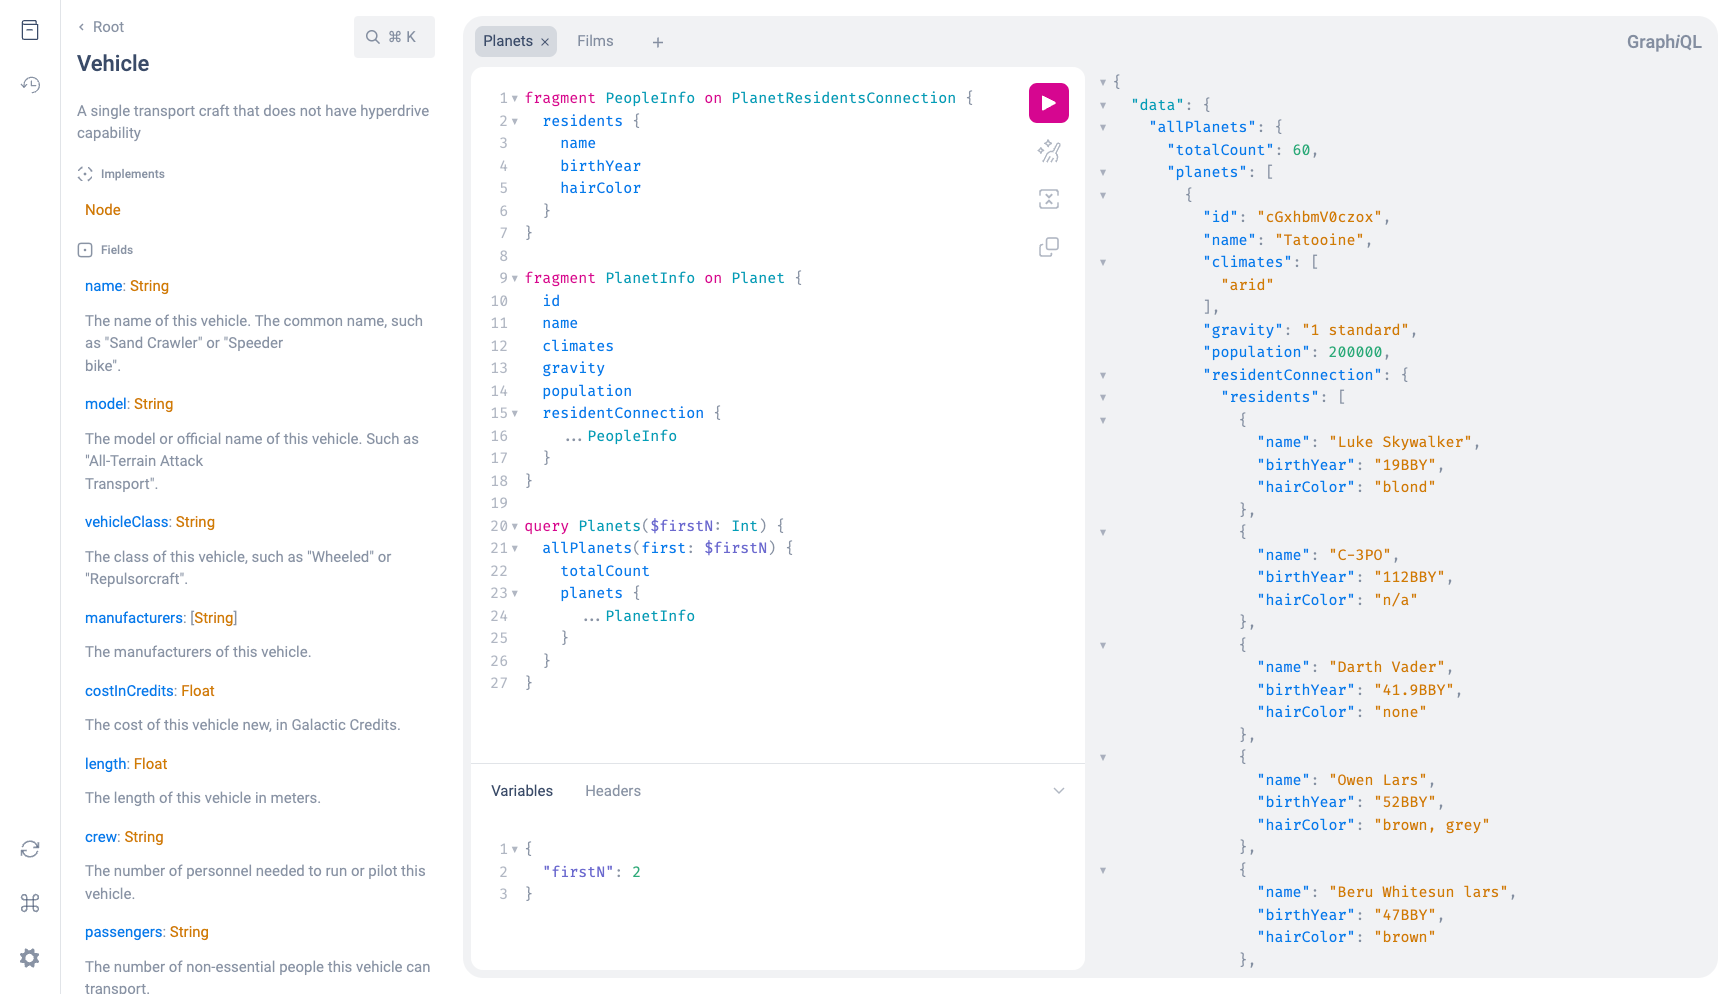
\includegraphics[width=0.8\textwidth]{images/graphql/graphiql}
    \caption{GraphiQL UI~\cite{graphql-graphiql}}
    \label{fig:graphql-graphiql}
\end{figure}

The main features are:
\begin{itemize}
    \item static website,
    \item documentation with comments,
    \item listing of queries, mutations, and types,
    \item execution of queries and mutations,
    \item autocompletion,
    \item metadata support~\cite{graphql-graphiql}.
\end{itemize}

The main disadvantages (compared to my task) are:
\begin{itemize}
    \item disconnection between documentation and query execution,
    \item requires manual implementation - library usage~\cite{graphql-graphiql}.
\end{itemize}

\subsection{RESTful API}
In the RESTful API world, there are several tools for generating documentation or interactive calls.
Swagger UI is one of the most popular ones, which I will mainly cover and compare with the gRPC options.

\subsubsection{ReDoc}
ReDoc is a tool for generating documentation based on the definition of OpenAPI.
It is a static website with a responsive layout.
It is used to preview documentation comments with example requests and responses and to show implementation examples.
The UI is in the figure~\ref{fig:rest-redoc}.
\cite{rest-redoc}

\begin{figure}[hbt!]
    \centering
    \captionsetup{justification=centering}
    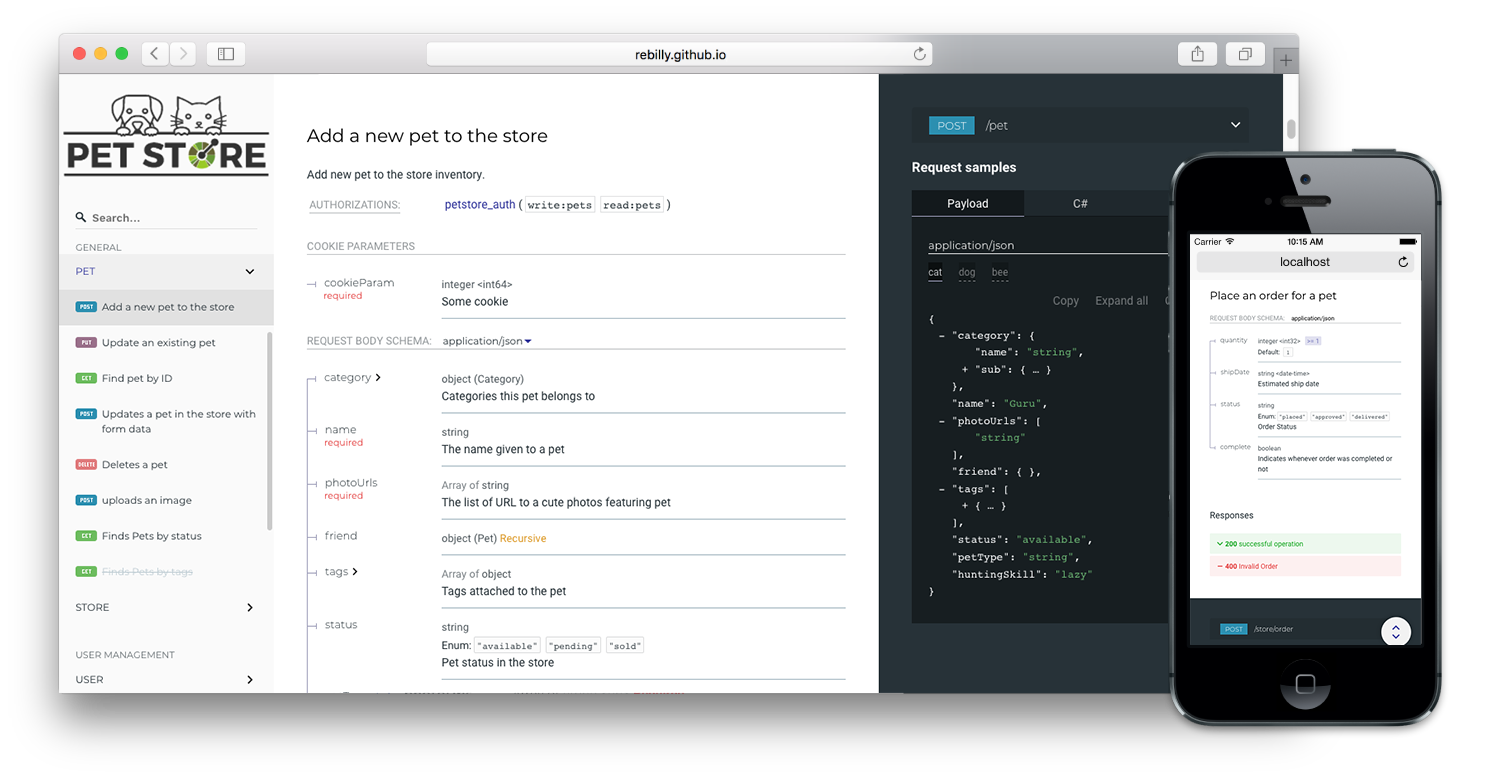
\includegraphics[width=0.8\textwidth]{images/rest/redoc}
    \caption{ReDoc UI~\cite{rest-redoc}}
    \label{fig:rest-redoc}
\end{figure}

The main features are:
\begin{itemize}
    \item static website,
    \item responsive layout,
    \item documentation with comments,
    \item preview example requests and responses,
    \item implementation examples~\cite{rest-redoc}.
\end{itemize}

The main disadvantage (compared to my task) is no option of calling the endpoints~\cite{rest-redoc}.

\subsubsection{RapiDoc}
RapiDoc is interactive API documentation with OpenAPI definition.
It is a static website, supports documentation comments, and allows calling the endpoints.
The UI is in the figure~\ref{fig:rest-rapidoc}.
\cite{rest-rapidoc}

\begin{figure}[hbt!]
    \centering
    \captionsetup{justification=centering}
    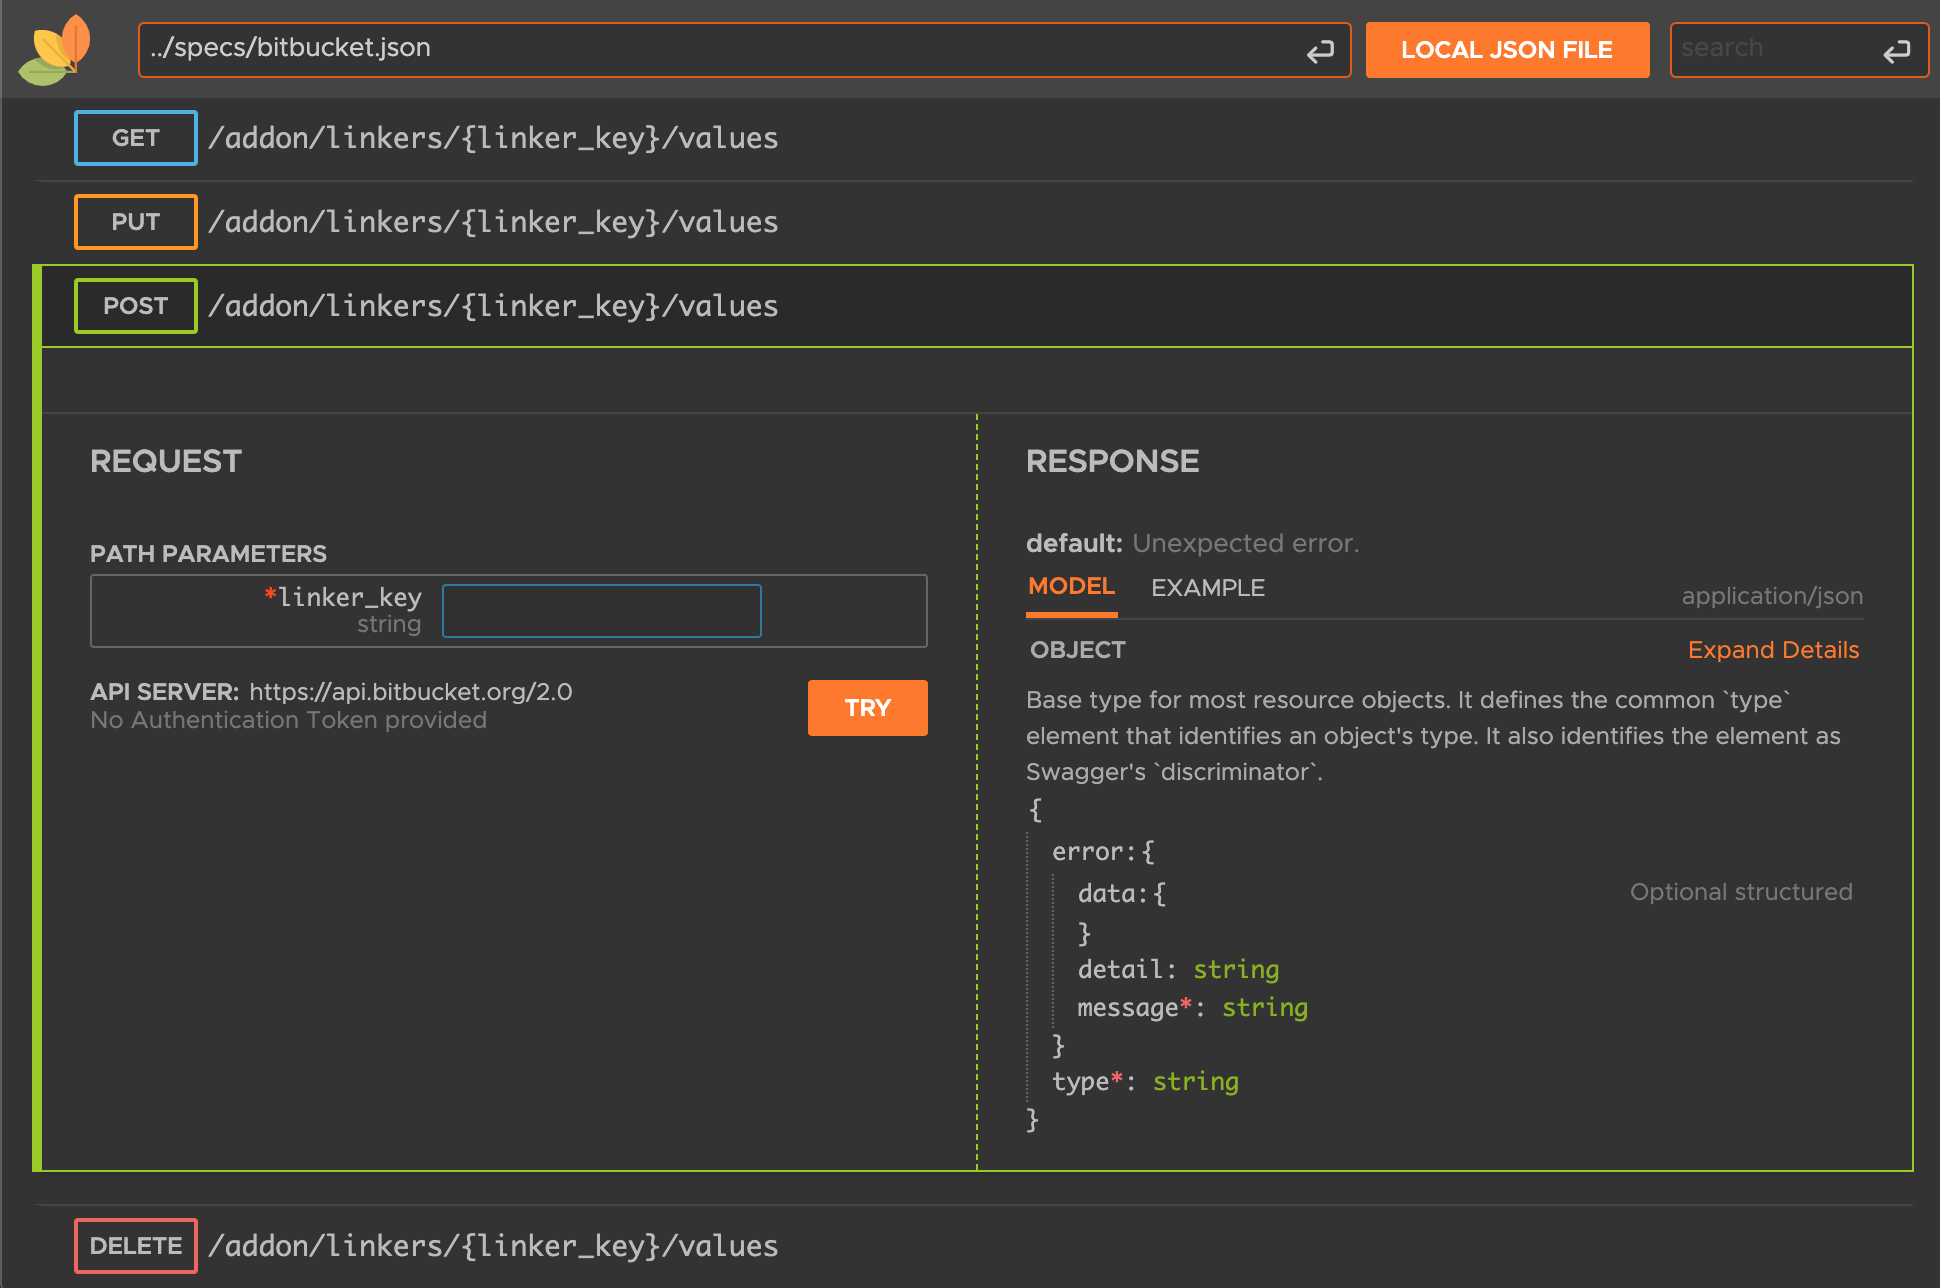
\includegraphics[width=0.8\textwidth]{images/rest/rapidoc}
    \caption{RapiDoc UI~\cite{rest-rapidoc}}
    \label{fig:rest-rapidoc}
\end{figure}

The main features are:
\begin{itemize}
    \item static website,
    \item documentation with comments,
    \item preview example requests and responses,
    \item implementation examples,
    \item ability to call endpoints,
    \item support for metadata,
    \item support for authentication mechanisms~\cite{rest-rapidoc}.
\end{itemize}

I have not found any main disadvantages (compared to my task) of RapiDoc.

\subsubsection{Swagger UI}
Swagger UI is one of the most popular choices for RESTful API documentation~\cite{rest-swagger-ui-popularity}.
The parent project is OpenAPI, a specification for general building HTTP APIs.
This tool is used to generate documentation from the OpenAPI definition.
It is a static website with support for comments and interactive endpoint calling.
The UI is in the figure~\ref{fig:rest-swagger-ui}.
\cite{rest-swagger-ui}

\begin{figure}[hbt!]
    \centering
    \captionsetup{justification=centering}
    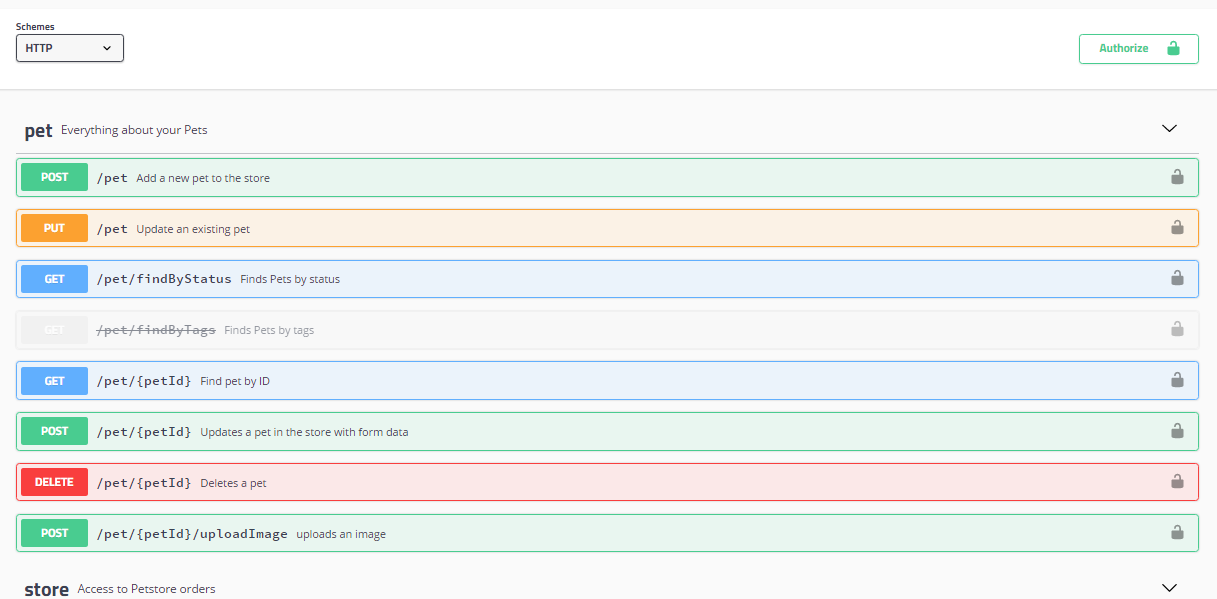
\includegraphics[width=0.8\textwidth]{images/rest/swagger-ui}
    \caption{Swagger UI~\cite{rest-swagger-ui}}
    \label{fig:rest-swagger-ui}
\end{figure}

The main features are:
\begin{itemize}
    \item static website,
    \item documentation with comments,
    \item preview example requests and responses,
    \item implementation examples,
    \item ability to call endpoints,
    \item support for metadata,
    \item support for authentication mechanisms~\cite{rest-swagger-ui}.
\end{itemize}

I have not found any main disadvantages (compared to my task) of Swagger UI\@.

\subsection{Summary}
I have compiled main tools for documenting and interacting with Protocol Buffers, GraphQL, and RESTful APIs.
For each tool, I have described the overall image and the main features and disadvantages.
While many of them excel in certain areas, they often fail to provide an experience that combines documentation rendering and interactive API exploration.
The comparison of the main features of the Protocol Buffers tools is in the table~\ref{tab:grpc-comparison-table}.

\begin{landscape}
    \begin{table}[]
        \centering
        \resizebox{\columnwidth}{!}{%
            \begin{tabular}{|l|l|l|l|l|l|l|l|l|l|l|}
                \hline
                & \textbf{Wombat} & \textbf{BloomRPC} & \textbf{gRPC Docs} & \textbf{gRPC UI} & \textbf{letmegrpc} & \textbf{gRPC-swagger} & \textbf{gRPC-Gateway} & \textbf{Postman} & \textbf{proto2asciidoc} & \textbf{protoc-gen-doc} \\ \hline
                Type                                 & Desktop App     & Desktop App       & Static Web         & Website          & Website              & Website               & Proxy                 & Desktop App & AsciiDoc & Static Web, JSON \\ \hline
                Listing of services \& methods       & x               & x                 & x                  & x                &                      & x                     &                       & x                & x                       & x                       \\ \hline
                Input as form                        & x               &                   &                    & x                & x                    &                       &                       &                  &                         &                         \\ \hline
                Input as JSON                        &                 & x                 &                    & x                &                      & x                     &                       & x                &                         &                         \\ \hline
                Request metadata                     & x               & x                 &                    & x                &                      & x                     & x                     & x                &                         &                         \\ \hline
                Headers \& Trailers                  & x               &                   &                    & x                &                      & x                     & x                     & x                &                         &                         \\ \hline
                Execution of requests                & x               & x                 &                    & x                & x                    & x                     & x                     & x                &                         &                         \\ \hline
                Determine schema via gRPC reflection & x               &                   &                    & x                &                      & x                     & x                     & x                & ? (not specified)       & ? (not specified)       \\ \hline
                Schema from .proto files             & x               & x                 & x                  & x                & x                    &                       & x                     & x                &                         &                         \\ \hline
                Documentation comments               &                 &                   &                    &                  & $\sim$ (in tooltips) &                       &                       &                  & x                       & x                       \\ \hline
                Maintained                           &                 &                   &                    & x                &                      &                       & x                     & x                &                         & x                       \\ \hline
            \end{tabular}%
        }
        \caption{Protocol Buffers Comparison Table}
        \label{tab:grpc-comparison-table}
    \end{table}
\end{landscape}

For Protocol Buffers, the most dominant are desktop applications like Wombat, BloomRPC, and Postman, which facilitate the browsing and calling of gRPC services.
However, these applications generally lack support for rendering documentation comments or determining gRPC schema via reflection.
Web-based solutions like gRPC Docs, gRPC UI, letmegrpc, and gRPC-swagger offer interactive gRPC calling capabilities.
Still, they frequently encounter limitations like interactive streaming support, documentation comments integration, or special server setup requirements.
This means developers must set up and maintain a server infrastructure specifically for API documentation and interaction.
Additionally, static documentation generators like proto2asciidoc or protoc-gen-doc can render comments from .proto files as markup, but they do not allow direct interaction with the services.
The gRPC-Gateway is a unique tool that generates a reverse proxy server for translating HTTP JSON APIs into gRPC\@.
While it is not directly comparable to the other tools, it is worth mentioning due to its ability to generate OpenAPI definitions, which can be used with existing tools for HTTP APIs.
Also, I think it is important to point out that maintenance of the tools is generally not good, with most of them being inactive for more than a year.
Only gRPC UI, gRPC-Gateway, protoc-gen-doc, and Postman are actively maintained.
Overall, the combination of having a static website with documenting comments and being able to call specific service methods interactively is lacking in current gRPC tools.

In the GraphQL realm, a documentation-focused tool, graphdoc generates static documentation websites from schema definitions, providing a comprehensive view of the available queries, mutations, and types.
However, this tool cannot execute queries and mutations, limiting its usefulness for interactive API exploration.
On the other hand, GraphQL Playground and GraphiQL are powerful web IDEs that do not require a specific server to be running and excel in executing queries and mutations.
Still, they struggle to integrate documentation seamlessly and comprehensively in their UI, where only GraphiQL includes the documentation comments but is not able to connect them with the queries directly.
As a result, none of the most popular tools I have found combine comprehensive documentation rendering with fully interactive query capabilities in a static website format.

In contrast, the RESTful API ecosystem is in a vastly different state.
The ReDoc tool is a static website generator that renders documentation from OpenAPI definitions, providing a view of the available endpoints, request/response examples, and implementation examples.
However, it does not support interactive API execution.
On the other hand, solutions like Swagger UI and RapiDoc render documentation from OpenAPI definitions while allowing interactive API execution.
These tools provide a cohesive experience for developers working with RESTful APIs, blending documentation and interaction capabilities while being able to run as a static website.
I have found no significant disadvantages to either of these tools.

\subsubsection{Comparison}
Comparing the tools for Protocol Buffers, GraphQL, and RESTful APIs, I have found that the RESTful API tools are the most advanced in terms of combining documentation rendering with interactive API exploration.
Tools like Swagger UI and RapiDoc provide a cohesive experience for developers working with RESTful APIs, blending documentation and interaction capabilities while being able to run a static website.
They have features like listing endpoints, input as form or JSON (in a combined way, where the form is only to a first level of hierarchy deepness), request/response metadata, execution of requests, and documentation comments.

The GraphQL tools are also quite advanced, but they often struggle with integrating documentation comments into the interactive query execution.
The Protocol Buffers tools are the least advanced, with most tools focusing on either documentation rendering or interactive API exploration, but not both.
Also, the maintenance of the tools is generally not good, with most of them being inactive for more than a year.

\subsubsection{Issues}
Despite the strengths of existing tools for Protocol Buffers, there remains a notable gap for an integrated solution that can cater to a unified static web generator that can provide a cohesive experience by combining documentation and fully interactive request/response capabilities with support for features like streaming, headers and trailers metadata.
This website generator should be able to create the static website from .proto files or gRPC reflection.

The main issues I will be addressing are:
\begin{itemize}
    \item documentation comments,
    \item interactive streaming,
    \item gRPC reflection,
    \item request metadata, headers, and trailers.
\end{itemize}


\section{Requirements}
The main requirement is to create a static website documentation for Protocol Buffers, which supports API calls.
The website should be able to render documentation comments, list services and methods, execute requests, and support request metadata, headers, and trailers.
It has to understand all gRPC features like messages, services, methods, and enums.
The website should be generated from .proto files or gRPC reflection.

Based on the issues and primary features described previously in the tools, I have compiled functional and non-functional requirements covering the required functionality of the static website interactive documentation generator.

\subsection{Functional Requirements}
% What should the system do
\newcounter{fcounter}
\newcommand{\functional}[1]{%
    \stepcounter{fcounter}%
    \subsubsection{F\arabic{fcounter} -- #1}%
}

\functional{List services and methods}
The website should list all services and methods available in the Protocol Buffers.

\functional{List message types}
The website should list all message types available in the Protocol Buffers.

\functional{List enum types}
The website should list all enum types available in the Protocol Buffers.

\functional{Show comments for services, methods, message types, and enum types}
Comments from the Protocol Buffers definitions should be rendered in the website for services, methods, message, and enum types.

\functional{Show comments for fields}
Comments from the Protocol Buffers definitions should be rendered in the website for fields in message or enum types.

\functional{Execution of methods with unary requests}
The website should allow for the execution of unary requests.

\functional{Execution of methods with server streaming requests}
The website should allow for the execution of server streaming gRPC method requests.
Also, streaming cancellation should be allowed in the middle of the execution.

\functional{Request body message input}
The website should allow request data input as a form or JSON\@.
It has to support all scalar types, including bytes and enums.
The input should also contain an example of the message structure.

\functional{Input form validation for the correct message structure}
The website should validate the input form for the correct message structure and show an error if the structure is incorrect.

\functional{Request metadata input}
The website should allow for input of request metadata.

\functional{Response headers and trailers}
The website should show response headers and trailers.

\functional{Response message}
The website should display the response message or messages.

\functional{Support for oneof fields}
The website should support oneof the fields in the message types.
They must be supported in the input request and the message definition.

\functional{Support for map fields}
The website should support map fields in the message types.
They must be supported in the input request and the message definition.

\functional{Support for repeated fields}
The website should support repeated fields in the message types.
They must be supported in the input request and the message definition.

\functional{Support for nested messages}
The website should support nested messages in the message types.
They must be supported in the input request and the message definition.

\functional{Support for well-known types}
The website should support well-known types like Timestamp, Duration, FieldMask, etc.
They must be supported in the input request and the message definition.

\functional{Generate website from .proto files}
The generator should be able to generate the website from .proto files.
The .proto files can be a single file or a folder.

\functional{Generate a website from gRPC reflection}
The generator should be able to generate the website from gRPC reflection.
The reflection can be from a server or a protoset definition file.

\functional{Global metadata and authorization}
The website should allow for global metadata definition and authorization metadata.
It should be possible to set the metadata for all requests and methods.

\functional{Options should be shown}
The website should show the options for services and methods.

\subsection{Non-Functional Requirements}
\newcounter{nfcounter}
\newcommand{\nonfunctional}[1]{%
    \stepcounter{nfcounter}%
    \subsubsection{N\arabic{nfcounter} -- #1}%
}

\nonfunctional{Static Website}
The website should be static.
It means only a combination of static files like HTML, CSS, and JavaScript without requiring a dynamic server to be run.
This should allow for easy deployment and hosting on various platforms.

\nonfunctional{Familiar UI}
The website should have a familiar UI for developers, probably close to something already used in the RESTful or GraphQL worlds.
It should be easy to navigate and understand, with a clear structure and layout.

\nonfunctional{Input as form or JSON}
The website should allow request data input as a form or JSON\@.
Depending on the developer's preference, this should allow for flexibility in how the data is entered.


\section{Use Cases}
Based on the requirements and comparing the existing tools, I have compiled a list of use cases that the static website interactive documentation generator should support.
The figure~\ref{fig:use-case-diagram} shows the diagram of the use cases and their relationships with the actors.
% TODO: How many actors?
In my case, I have two actors.
One is the Application Developer, who uses the website to explore and interact with the gRPC services.
The other is the gRPC Developer, who generates the static website from the .proto files or gRPC reflection.

\begin{figure}
    \centering
    \captionsetup{justification=centering}
    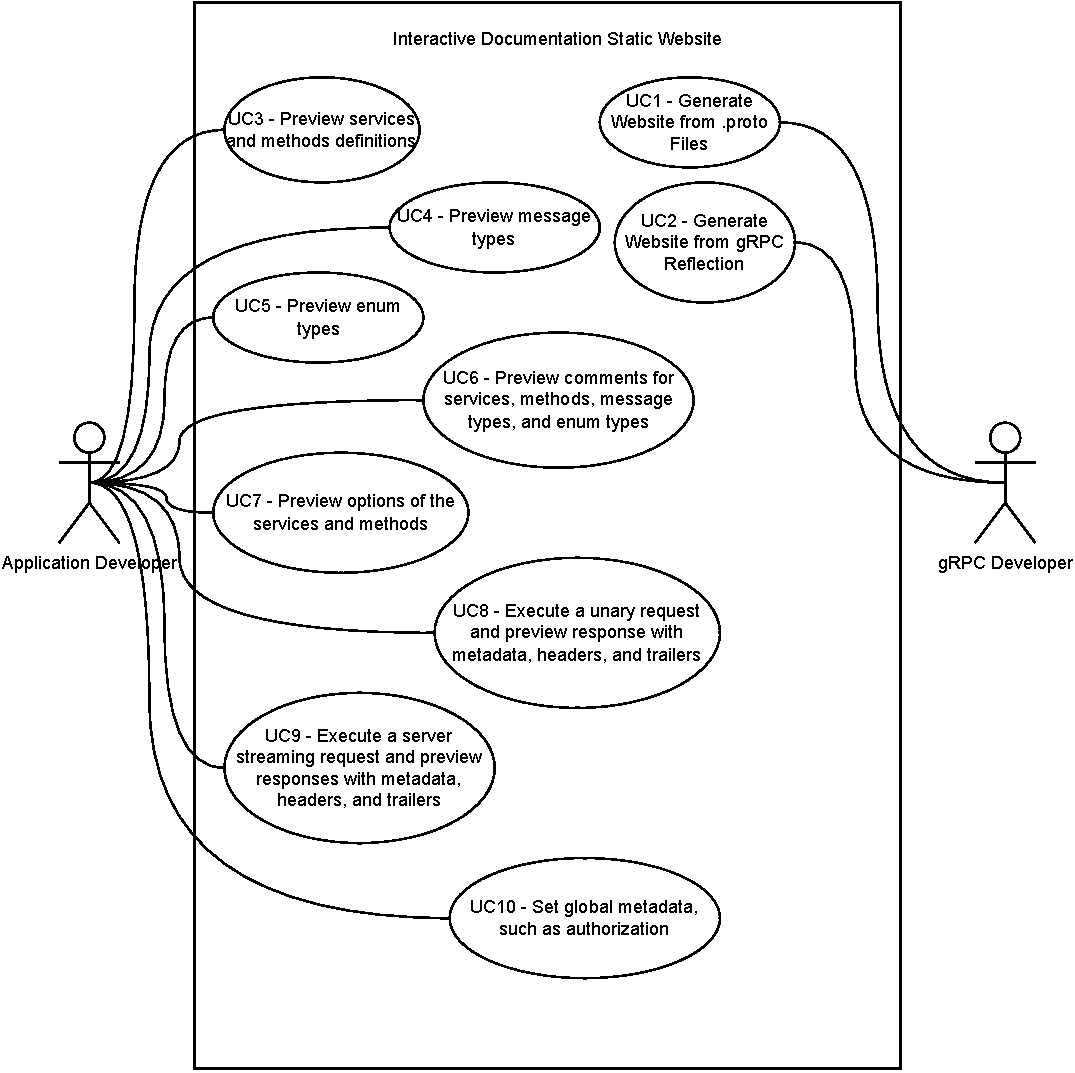
\includegraphics[width=1.0\textwidth]{images/use-case-diagram}
    \caption{Use Case Diagram}
    \label{fig:use-case-diagram}
\end{figure}


\newcounter{uccounter}
\newcommand{\usecase}[2]{%
    \stepcounter{uccounter}%
    \subsection{UC\arabic{uccounter} -- #1}
}


\usecase{Generate Website from .proto Files}

\textbf{Primary Actor:} gRPC Developer\\
\textbf{Preconditions:} The gRPC Developer has the .proto files ready.
Either as separate files in a folder or as interlinked files using imports.\\
\textbf{Goal:} The website is generated.\\
\textbf{Main Scenario:}
The gRPC Developer runs the generator.
The generator reads the .proto files.
The generator generates the website's necessary files for these definitions.
The website is ready for the gRPC Developer to be hosted.\\
\textbf{Alternative Scenario 1:}
The generator finds an error when parsing the .proto files.
So, it shows an error message to the gRPC Developer.
The gRPC Developer has to fix the error in the .proto files and rerun the generator.\\
\textbf{Alternative Scenario 2:}
The .proto files do not exist.
The generator shows an error message to the gRPC Developer.
The gRPC Developer has to provide the .proto files and rerun the generator.

\usecase{Generate Website from gRPC Reflection}

\textbf{Primary Actor:} gRPC Developer\\
\textbf{Preconditions:} The gRPC Developer has the gRPC server with reflection enabled, ready and running.\\
\textbf{Goal:} The website is generated.\\
\textbf{Main Scenario:}
With reflection enabled, the gRPC Developer runs some tools to get the Protocol Buffer definitions from the target gRPC server.
After the Protocol Buffer definitions are created, the gRPC Developer runs the generator and feeds it the definitions.
The generator reads the definitions and generates the website's necessary files.
The website is ready for the gRPC Developer to be hosted.\\
\textbf{Alternative Scenario 1:}
The generator finds an error when parsing the definitions file.
So, it shows an error message to the gRPC Developer.
The gRPC Developer has to regenerate the definitions file and rerun the generator.\\
\textbf{Alternative Scenario 2:}
The definition file does not exist.
The generator shows an error message to the gRPC Developer.
The gRPC Developer has to provide the definition file and rerun the generator.


\usecase{Preview services and methods definitions}

\textbf{Primary Actor:} Application Developer\\
\textbf{Preconditions:} The Application Developer has opened the static website with the Protocol Buffers definition defined.\\
\textbf{Goal:} The services and methods are shown.\\
\textbf{Main Scenario:}
The Application Developer opens the website.
The website shows the services and methods available in the definitions of Protocol Buffers.
The Application Developer can see the details of the services and methods with their relevant package paths.\\
\textbf{Alternative Scenario 1:}
The website does not show the services and methods.
The Application Developer sees an error message or empty page.
The Application Developer has to ask the gRPC Developer to check the Protocol Buffers definitions and regenerate the website.

\usecase{Preview message types}

\textbf{Primary Actor:} Application Developer\\
\textbf{Preconditions:} The Application Developer has opened the static website with the Protocol Buffers definition defined.\\
\textbf{Goal:} The message types are shown.\\
\textbf{Main Scenario:}
The Application Developer opens the website.
The website shows the message types available in the definitions of Protocol Buffers.
The Application Developer can see the details of the message type with their fields and nested message types.\\
\textbf{Alternative Scenario 1:}
The website does not show the message types.
The Application Developer sees an error message or empty page.
The Application Developer has to ask the gRPC Developer to check the Protocol Buffers definitions and regenerate the website.

\usecase{Preview enum types}

\textbf{Primary Actor:} Application Developer\\
\textbf{Preconditions:} The Application Developer has opened the static website with the Protocol Buffers definition defined.\\
\textbf{Goal:} The enum types are shown.\\
\textbf{Main Scenario:}
The Application Developer opens the website.
The website shows the enum types available in the definitions of Protocol Buffers.
The Application Developer can see the details of the enum type with their keys and values.\\
\textbf{Alternative Scenario 1:}
The website does not show the enum types.
The Application Developer sees an error message or empty page.
The Application Developer has to ask the gRPC Developer to check the Protocol Buffers definitions and regenerate the website.

\usecase{Preview comments for services, methods, message types, and enum types}

\textbf{Primary Actor:} Application Developer\\
\textbf{Preconditions:} The Application Developer has opened the static website with the Protocol Buffers definition defined.\\
\textbf{Goal:} The comments are shown.\\
\textbf{Main Scenario:}
The Application Developer opens the website.
The website shows all defined comments for services, methods, message types, and enum types.
The Application Developer can see all the comments for each of them.\\
\textbf{Alternative Scenario 1:}
The website does not show the defined comments.
The Application Developer sees an error message or no comments on the page.
The Application Developer has to ask the gRPC Developer to check the Protocol Buffers definitions and regenerate the website.

\usecase{Preview options of the services and methods}

\textbf{Primary Actor:} Application Developer\\
\textbf{Preconditions:} The Application Developer has opened the static website with the Protocol Buffers definition defined.\\
\textbf{Goal:} The options are shown.\\
\textbf{Main Scenario:}
The Application Developer opens the website.
The website shows all defined options for services and methods.
The Application Developer can see the last defined options for each of them.\\
\textbf{Alternative Scenario 1:}
The website does not show the defined options.
The Application Developer sees an error message or no options on the page.
The Application Developer has to ask the gRPC Developer to check the Protocol Buffers definitions and regenerate the website.

\usecase{Execute a unary request and preview response with metadata, headers, and trailers}

\textbf{Primary Actor:} Application Developer\\
\textbf{Preconditions:} The Application Developer has opened the static website with the Protocol Buffers definition defined.\\
\textbf{Goal:} Execution is successful, and the response is shown.\\
\textbf{Main Scenario:}
The Application Developer opens the website.
First, they define the target server URL\@.
Then, they select a service and method.
They fill in the request data and metadata.
They execute the request.
The website shows headers, then the response, and finally, the trailers.\\
\textbf{Alternative Scenario 1:}
The request data are invalid.
The website shows an error message.
The Application Developer has to fix the request data and rerun the request.\\
\textbf{Alternative Scenario 2:}
The request fails for any reason.
The website shows an error message.
The Application Developer has to check the server status, the request data, and metadata and rerun the request.\\
\textbf{Alternative Scenario 3:}
The request is taking too long.
The Application developer can cancel the request in the middle of the execution.
They have to check the server status, the request data, and metadata and rerun the request.

\usecase{Execute a server streaming request and preview responses with metadata, headers, and trailers}

\textbf{Primary Actor:} Application Developer\\
\textbf{Preconditions:} The Application Developer has opened the static website with the Protocol Buffers definition defined.\\
\textbf{Goal:} Execution is successful, and all responses are shown.\\
\textbf{Main Scenario:}
The Application Developer opens the website.
First, they define the target server URL\@.
Then, they select a service and method.
They fill in the request data and metadata.
They execute the request.
The website shows headers, then all responses while they are arriving from the server one by one, and finally, trailers.\\
\textbf{Alternative Scenario 1:}
The request data are invalid.
The website shows an error message.
The Application Developer has to fix the request data and rerun the request.\\
\textbf{Alternative Scenario 2:}
The request fails for any reason.
The website shows an error message.
The Application Developer has to check the server status, the request data, and metadata and rerun the request.\\
\textbf{Alternative Scenario 3:}
The request is taking too long.
The Application developer can cancel the request in the middle of the execution.
They have to check the server status, the request data, and metadata and rerun the request.

\usecase{Set global metadata, such as authorization}

\textbf{Primary Actor:} Application Developer\\
\textbf{Preconditions:} The Application Developer has opened the static website with the Protocol Buffers definition defined.\\
\textbf{Goal:} Execution is successful, and the global metadata is included in the request.\\
\textbf{Main Scenario:}
The Application Developer opens the website.
First, they define the target server URL\@.
Then, they select a service and method.
They fill in the request data and metadata.
They execute the request.
The website shows the executed request containing the global metadata.


\section{Requirements to Use Cases Mapping}
I have compiled a table of requirements and use cases mapping (see table~\ref{tab:use_cases}) to verify that all requirements are covered by at least one use case and that no use case is unnecessary.
The table shows that all requirements are covered.

\begin{table}[hbt!]
    \centering
    \captionsetup{justification=centering}
    \begin{tabular}{|l|l|l|l|l|l|l|l|l|l|l|}
        \hline
        & \multicolumn{10}{c|}{\textbf{Use Cases}} \\ \hline
        & 1 & 2 & 3 & 4 & 5 & 6 & 7 & 8 & 9 & 10 \\ \hline
        F1  &   &   & x &   &   &   &   &   &   &    \\ \hline
        F2  &   &   &   & x &   &   &   &   &   &    \\ \hline
        F3  &   &   &   &   & x &   &   &   &   &    \\ \hline
        F4  &   &   &   &   &   & x &   &   &   &    \\ \hline
        F5  &   &   &   &   &   & x &   &   &   &    \\ \hline
        F6  &   &   &   &   &   &   &   & x &   &    \\ \hline
        F7  &   &   &   &   &   &   &   &   & x &    \\ \hline
        F8  &   &   &   &   &   &   &   & x & x &    \\ \hline
        F9  &   &   &   &   &   &   &   & x & x &    \\ \hline
        F10 &   &   &   &   &   &   &   & x & x &    \\ \hline
        F11 &   &   &   &   &   &   &   & x & x &    \\ \hline
        F12 &   &   &   &   &   &   &   & x & x &    \\ \hline
        F13 &   &   &   & x &   &   &   & x & x &    \\ \hline
        F14 &   &   &   & x &   &   &   & x & x &    \\ \hline
        F15 &   &   &   & x &   &   &   & x & x &    \\ \hline
        F16 &   &   &   & x &   &   &   & x & x &    \\ \hline
        F17 &   &   &   & x &   &   &   &   &   &    \\ \hline
        F18 & x &   &   &   &   &   &   &   &   &    \\ \hline
        F19 &   & x &   &   &   &   &   &   &   &    \\ \hline
        F20 &   &   &   &   &   &   &   &   &   & x  \\ \hline
        F21 &   &   &   &   &   &   & x &   &   &    \\ \hline
    \end{tabular}%
    \caption{Requirements to Use Cases Mapping}
    \label{tab:use_cases}
\end{table}